% !TEX root = approx8.tex

\newpage

\section{Abouzaid's splitting principle in the filtered case and approximability} \label{sec:split-app}
In this section we prove the second and third points in Theorem \ref{thmmain1}. To this aim, we establish a persistence version of the split-generation criterion due to Abouzaid \cite{Ab:geom-crit} (for the closed monotone case see \cite{she:fanofuk}). The key point is that the energy cost of reaching the unit in the quantum homology of the ambient symplectic manifold through the open-closed map can be directly interpreted in terms of  retract  approximability, as defined in Chapter \ref{ch:prelim}.  We provide two examples of computations, completing the proof of Theorem \ref{thmmain1}. 
Along the way,  we adjust to this persistence setting the various
ingredients in Abouzaid's result, namely the open-closed and closed open maps and their relation to a persistence version of Hochschild homology.


%We briefly recall the definition of the ambient quantum homology $QH(X)$ of $M$. Consider the monotone family $\lagmon$, a finite subfamily $\mathcal{B}$ {\color{purple} Not sure about the notation for the subfamily.}. Fix for the moment a perturbation datum $p\in \mathcal{P}$ and consider the monotone Fukaya category $\fuk(\lagmon;p)$.
%=======================================
%=======================================
%=======================================

\subsection{The results}
Let $(X,\omega)$ be a monotone symplectic manifold. We recall that given a Novikov element $\mathbf{d} \in \Lambda_0$, then $\lagmon$ is the collection of closed, graded and monotone Lagrangians $L = (\overline{L}, a_L, s_L)$ with Maslov-$2$ disk count equal to $\mathbf{d}$. We fix a choice of $\mathbf{d}\in \Lambda_0$ for the rest of this chapter. Recall that we associated with $\lagmon$ a homotopy system of $A_\infty$-categories (see \S\ref{sbsb:homotopy-sys} for the definition) $\widehat{\fuk}(\lagmon)$ indexed by the space $\mathcal{P}$ of perturbation data, such that each filtered and strictly unital $A_\infty$-category $\fuk(\lagmon;p)$, $p\in \mathcal{P}$, has $\lagmon$ as set of objects. We will often abbreviate and write the system as $\widehat{\mathcal{A}}:=\widehat{\fuk}(\lagmon)$ and each component as 
$$\mathcal{A}_p:= \fuk(\lagmon;p)~.~$$ We omit the manifold $X$ from the notation as it is also fixed for the remainder of the section.

A subset $\mathcal{B}\subset \lagmon$ induces a full $A_\infty$-subcategory $\mathcal{B}_p$ of $\mathcal{A}_p$ for any perturbation datum $p\in \mathcal{P}$. This  ultimately leads to a subsystem $\widehat{\mathcal{B}}$ of $\widehat{\mathcal{A}}$. %{\color{red} Moreover, $\mathcal{B}_p$ induces a filtered $\mathcal{A}_p$-bimodule $\overline{\mathcal{B}_p}$ as explained above in \S\ref{WRSG} {\huge to move somewhere else}}.

The following geometric criterion for retract approximability,
in the sense of Definition \ref{d:approx-sys-ret} with $\lagmon \subset \text{Obj}(\widehat{\mathcal{A}})$, is the main result 
of the section.

\begin{thm}\label{gio:wabomain}
	Let $\epsilon>0$. If there is a finite subset $\mathcal{F}_\epsilon\subset\lagmon$ such that the colimit persistence open-closed map $$\widehat{OC}\colon PHH_*(\widehat{\mathcal{F}_\epsilon})\to QH^{*+n}(X,\Lambda)_{\mathbf{d}}$$ satisfies $$i_{0,\epsilon}(u_{\mathbf{d}})\in \text{image}\left(PHH^\epsilon(\widehat{\mathcal{F}_\epsilon})\to QH^\epsilon(X,\Lambda)_{\mathbf{d}}\right)$$ where $u_\mathbf{d}\in QH^0(X,\Lambda)_\mathbf{d}$ is the projection of the quantum cohomology unit  $u\in QH(X,\Lambda)$ to $QH(X,\Lambda)_\mathbf{d}$ and $i_{0,\epsilon}$ is part of the structure maps of the quantum cohomology persistence module, then $\lagmon$ is $\frac{\epsilon}{2}$-retract-approximable by $\mathcal{F}_\epsilon$ in $PD(\widehat{\fuk}(\lagmon))$.
\end{thm}
\noindent The open closed map $OC$, the sense in which we take a colimit, and the various other notions appearing in the statement of Theorem \ref{gio:wabomain} and its proof, among them, the persistence Hochschild homology $PHH( - )$, will be made explicit below.
%One should think of it as the open closed map associated with the %Fukaya category with full accuracy (see discussion at the %beginning of \S\ref{s:sys-tpc}).
We now restate the points $(ii)$ and $(iii)$ of Theorem \ref{thmmain1} as corollaries of Theorem \ref{gio:wabomain}.
\begin{cor}\label{S2T2}
The classes $\lag^{\text{(mon,} \mathbf{0} \text{)}}(S^2)$ and $\lagwex(\mathbb{T}^2)$ are TPC retract approximable.
\end{cor}
\noindent The proof of Theorem \ref{gio:wabomain} is contained in \S\ref{gio:proofwabomain}. The proof of Corollary \ref{S2T2} occupies \S\ref{gio:proofS2T2}. The proof of the last two points of Theorem \ref{thmmain1} follows directly from this Corollary and is concluded in \S\ref{subsec:proof_ThmAii}.

%=======================================
%=======================================
%=======================================


\subsection{Proof of Theorem \ref{gio:wabomain}}\label{gio:proofwabomain}
We split the proof of Theorem \ref{gio:wabomain} into several steps. \S\ref{WRSG} contains a persistence version of Abouzaid's algebraic split-generation criterion. The main result, in Proposition \ref{gio:algfilabo}, shows that retract approximability 
is naturally present in that context.
% \S\ref{gio:ffuk} recalls some of the main technical ingredients in the definition of the filtered Fukaya categories $\fuk(\lagmon;p)$ following Chapter \ref{ch:ffuk} in sufficient detail so that,
 In Section \ref{gio:coproduct}, \ref {AQH}, \ref{gio:oc} we set-up in the persistence setting the main geometric constructions needed for the split-generation criterion. 
Finally, in \S\ref{gio:aboappr} we put the constructions together and prove Theorem \ref{gio:wabomain}.

\subsubsection{Retract approximability}\label{WRSG}
Let $\mathcal{A}$ be a filtered $A_{\infty}$-category over $\Lambda$, such as one of the filtered Fukaya categories $\A_{p}$ from the beginning of \S\ref{sec:split-app}, and
let $\mathcal{B}\subset \text{Obj}(\mathcal{A})$. We regard $\mathcal{B}$ as a full $A_\infty$-subcategory of $\mathcal{A}$. In contrast to our general conventions, we do not assume here that $\mathcal{B}$ is closed under shifts or translations. We define a filtered $(\mathcal{A},\mathcal{A})$-bimodule $\overline{\mathcal{B}}$, which will be called the $\mathcal{B}$-bar bimodule. For two objects, $A$ and $B$,  of $\mathcal{A}$, we set, with the notation in Appendix \ref{a:fil-ai},  $$\overline{\mathcal{B}}(A,B):=\mathcal{Y}^r(A)\otimes_\mathcal{B}\mathcal{Y}^l(B) = \bigoplus_{d\geq 0}\bigoplus_{L_0,\ldots, L_d\in  \text{Ob}(\mathcal{B})}\mathcal{A}(A,L_0,\ldots, L_d,B)~.~$$ 
Here $\mathcal{Y}^l$ and $\mathcal{Y}^r$ denote the left and right filtered Yoneda embeddings, defined in Appendix \ref{gio:fyon-def}, and we implicitly view $\mathcal{Y}^r(A)$ and $\mathcal{Y}^l(B)$ as $A_\infty$-modules over $\mathcal{B}$. The tensor product $\otimes_\mathcal{B}$ is the usual derived tensor product over $\mathcal{B}$. Note that $\mathcal{A}(A,B)$ is not a summand in $\overline{\mathcal{B}}(A,B)$. We will often write a pure tensor $\gamma_1\otimes a_1\otimes \cdots \otimes a_d\otimes \gamma_2 \in \mathcal{A}(A,L_0,\ldots, L_d,B)$ as $\vec{\gamma}$. The bar differential $\mu^{\text{bar}}_{0|1|0}$ (which we will also denote by $d_{\text{bar}}$) is defined via \begin{align*}\mu^{\text{bar}}_{0|1|0}(\vec{\gamma}):=& \sum_{i=0}^d\mu_{1+i}(\gamma_1,a_1,\ldots, a_i)\otimes a_{i+1}\otimes \cdots \otimes a_d\otimes \gamma_2\\ +& \sum_{i\leq j} \gamma_1\otimes a_1\otimes \cdots \otimes a_{i-1}\otimes \mu_{j-i}(a_i,\ldots, a_j)\otimes a_{j+1}\otimes \cdots\otimes a_d\otimes \gamma_2\\ +&\sum_{i=1}^{d+1} \gamma_1 \otimes a_1 \otimes \cdots \otimes a_{i-1}\otimes \mu_{d-i+2}(a_i,\dots, a_d,\gamma_2) \end{align*} while the higher operations $\mu^{\text{bar}}_{l|1|r}$ are defined via\begin{itemize}
	\item for $l\geq 1$ and $r=0$: \begin{align*}\mu^{\text{bar}}_{l|1|0}(x_1,\ldots, x_l, \vec{\gamma}) :=& \sum_{i=0}^{d}\mu_{l+i+1}(x_1,\ldots, x_l, \gamma_1,a_1,\ldots, a_i)\otimes a_{i+1}\otimes \cdots \otimes a_d\otimes \gamma_2 \end{align*}
	\item for $l=0$ and $r\geq 1$: \begin{align*} \mu^{\text{bar}}_{0|1|r}(\vec{\gamma},y_1,\ldots, y_r):= \sum_{i=1}^{d+1} \gamma_1\otimes a_1\otimes \cdots \otimes a_{i-1}\otimes \mu_{d+r-i+2}(a_i,\ldots, a_d,\gamma_2,y_1,\ldots, y_r) \end{align*}
	\item for $l,r\geq 1$: $\mu^{\text{bar}}_{l|1|r}=0$ \end{itemize}
It is straightforward to see that $\overline{\mathcal{B}}$ is filtered, since $\mathcal{A}$ is. 
There is an obvious length filtration \begin{equation}\label{eq:lengthfiltration}
F^N\overline{\mathcal{B}}(A,B)= \bigoplus_{d=0}^N\bigoplus_{L_0,\ldots, L_d\in \text{Ob}(\mathcal{B})}\mathcal{A}(A,L_0,\ldots, L_d,B), \quad N\geq 0,
\end{equation} which induces $A_\infty$-bimodules $F^N{\mathcal{B}}$. The $A_\infty$-structure maps on $\mathcal{A}$ induce a filtered morphism of $(\mathcal{A},\mathcal{A})$-bimodules $$\mu:=\mu^{\overline{\mathcal{B}}} \colon \overline{\mathcal{B}}\to \Delta_\mathcal{A}$$ in an obvious way, where $\Delta_\mathcal{A}$ stands for the diagonal bimodule of $\mathcal{A}$.

Let now $K\in \text{Obj}(\mathcal{A})$ and consider the filtered chain map 
\begin{equation}\label{eq:bimod_map1}
	\mu^{\overline{\mathcal{B}}} (K) :=\mu^{\overline{\mathcal{B}}}_{0|1|0}\colon \overline{\mathcal{B}}(K,K)\to \mathcal{A}(K,K) ~.~
\end{equation} 
Denote by $$[\mu^{\overline{\mathcal{B}}}(K)]\colon H(\overline{\mathcal{B}}(K,K))\to H(\mathcal{A}(K,K))$$ the morphism of persistence modules induced by $\mu^{\overline{\mathcal{B}}}(K).$

In the context above,  given an object $K$ of $\mathcal{A}$, we denote its strict unit by $e_K\in \mathcal{A}^{\leq 0 }(K,K)$ and by $[e_K]\in \hom_{PD(\mathcal{A})}^0(K,K)$ its homology class in the TPC $PD(\mathcal{A})$. 

Finally, before stating the main result, we need one more notion. 
Let $V$ and $W$ be persistence modules and $f\colon V\to W$ a persistence morphism. We will make use of a measurement that estimates the energy gap
separating an element in $W$ from the image of $f$. More precisely, for  $w\in W_{r}$, we put:
\begin{equation}\label{eq:en_gap}
	R(w,f):=\inf\left\{s\geq r \ \lvert \ \exists v\in V_s, \ f_s(v) = i_{r,s}^W(w)\right\}
\end{equation} where $i^W_{r,s}\colon W_r\to W_s$ denotes the persistence structure map for $W$. If $i_{r,s}^W(w)\notin \text{image}(f_s)$ for all $s\geq r$ we set $R(w,f)=\infty$. 

\ 

Below and in what follows we denote by $\mathcal{F}\mathbf{Ch}$ the filtered $dg$-category of filtered chain complexes over $\Lambda$, and by $\hfch$ its persistence homological category in cohomological degree $0$, which is a TPC (see \cite[Section 2.5.2]{BCZ:tpc}). We recall that in our conventions, a filtered chain complex over $\Lambda$ is a chain complex over $\Lambda$, filtered by an increasing sequence of $\Lambda_0$-subcomplexes indexed by the real line (see Appendix \ref{a:sb:fil-ai}).

\begin{prop}\label{gio:algfilabo}
	Let $K$ be an object of $\mathcal{A}$, $\mathcal{B}$ be a finite full $A_\infty$-subcategory of $\mathcal{A}$ and $\alpha\in \mathbb{R}_{\geq 0}$. The following statements are equivalent:
	\begin{enumerate}
		\item\label{(1)} The estimate $R([e_K],[\mu^{\overline{\mathcal{B}}}(K)])\leq \alpha$ holds.%{\color{red}, where $[e_K]\in \hom_{PD(\mathcal{A})}^0(K,K)$ is the class of the strict unit $e_K\in \mathcal{A}^{\leq 0}(K,K)$.}%The unit $[e_K]\in H(\mathcal{A}(K,K))$ is in the image of $[\mu^{\overline{\mathcal{B}}}(K)^{\leq \alpha}]$, 
		%\item The element $\eta_\alpha^K\in \text{hom}_{PD(\mathcal{A})^0}(\Sigma^\alpha K,K)$ lies in the image of the induced map $$\mu^{\overline{\mathcal{B}}}(K)^\alpha: H(\overline{\mathcal{B}}^{\leq \alpha}(K,K))\to \text{hom}_{PD(\mathcal{A})^0}(\Sigma^\alpha K,K),$$
		\item\label{(2)} The map $\mu^{\overline{\mathcal{B}}}(K)\in \text{hom}_{(\hfch)^0}(\overline{\mathcal{B}}(K,K), \mathcal{A}(K,K))$ is an $\alpha$-isomorphism in $\hfch$.%{\color{red}, the homotopy category of filtered chain complexes over $\k$ (see \cite[Example 2.22]{BCZ:tpc}),}%		{\color{red} Or in the category of persistence modules? no, this is not traingulated...}
		\item\label{(3)} The object $K$ is $\frac{\alpha}{2}$-retract-approximable in $PD(\mathcal{A})$ by the family $\text{Obj}(\mathcal{B})$.
	\end{enumerate}
	Moreover, each of the above statements holds for all objects $K$ of $\mathcal{A}$ if and only if the cone of $\mu^{\overline{\mathcal{B}}}(K)$ seen as a morphism of $(\mathcal{A},\mathcal{A})$-bimodules is $\alpha$-acyclic in $H^0(F\text{bimod}_{\mathcal{A}, \mathcal{B}})$.% {\color{orange} the homological category of the filtered $dg$-category of filtered $A_\infty$-bimodules over $\mathcal{A}$}.
\end{prop}

\begin{rem} 
	Note that by \cite[Lemma 2.85]{BCZ:tpc}, if one of the statements in Proposition \ref{gio:algfilabo} holds, then the interleaving distance in $\hfch$ between $\overline{\mathcal{B}}(K,K)$ and $\mathcal{A}(K,K)$ is $\leq \alpha$.
\end{rem}
%\begin{rem} 	To make computations easier, we will work with twisted complexes over the image of the (left) Yoneda embedding, as in \cite[Appendix A]{Ab:geom-crit}. This is possible as the Yoneda embedding is a filtered $A_\infty$-functor, so that the homotopy category of twisted complexes over Yoneda modules is TPC isomorphic to the image of the extended Yoneda embedding over twisted complexes (see \S\ref{extendedYoneda} and \cite{Se:book-fukaya-categ}). The lengthier version of these computations, working directly over $FTw\mathcal{A}$ is carried out in Appendix \ref{abouznomodules}. {\texttt{I guess that this (computations in FTwA) will not appear in the paper, but maybe its worth it to put somewhere (my thesis?)}} \end{rem}
Before proving Proposition \ref{gio:algfilabo}, we start with two simple auxiliary results that will be used in the proof.
Let $\mathcal{C}$ be a PC, and consider objects $R$ and $X$ of $\mathcal{C}$. The measurement $\dret(R,X)$ has been defined in (\ref{eq:d-rint}). We define  a similar measurement $d'_{\text{r-int}}$ via \begin{align*}
	d'_{\text{r-int}}(R,X):=\frac{1}{2}\inf\Bigl\{r_1+r_2\bigm|&\, r_1,r_2\geq 0, \, \exists \, \varphi: \Sigma^{r_1}R \longrightarrow X,  \, \exists
	\, \psi: \Sigma^{r_2}X
	\longrightarrow R \\ &
	\;\; \text{such that} \; \psi \circ \Sigma^{r_2} \varphi = \eta_{r_1+r_2}^R
	\Bigr\}.
\end{align*} Of course we have $$d'_{\text{r-int}}(R,X) \leq \dret(R,X)\leq2 d'_{\text{r-int}}(R,X).$$

In the proof of Proposition \ref{gio:algfilabo} it is more convenient to use  $d'_{\text{r-int}}$ instead of $d_{\text{r-int}}$.
This is possible because their shift-invariant versions agree:
\begin{lem} For any objects $R$ and $X$ of $\mathcal{C}$ we have
	$$\sdret(R,X) = \bar{d'}_{\text{r-int}}(R,X)$$ where $\bar{d'}_{\text{r-int}}$ is defined as in Chapter \ref{ch:prelim} but with $\sdret$ replaced by $ d'_{\text{r-int}}(R,X)$.
\end{lem} 
\begin{proof}
	Assume $d'_{\text{r-int}}(R,X)<r$. Let $\varphi: \Sigma^{r_1}R \longrightarrow X$ and $\psi: \Sigma^{r_2}X
	\longrightarrow R$ such that $\psi \circ \Sigma^{r_2} \varphi = \eta_{r_1+r_2}^R$ and $r_1+r_2=2r$. Assume (without loss of generality) that $r_1\geq r_2$ and define $\alpha :=\frac{r_1-r_2}{2}$. Note that $r-\alpha = r_2$ Then $\Sigma^{-\alpha}\varphi\colon \Sigma^{r}R\to \Sigma^{-\alpha}X$ and $\psi\colon \Sigma^{-\alpha+r}X\to R$ show that $\sdret(R,X)<r$. The opposite inequality is obvious.
\end{proof}



%The next lemma is immediate.

%\begin{lem}\label{ezlemma0}
%	Consider the following commutative square of persistence maps
%	\begin{equation}
%		\label{persistencediagram} \xymatrixcolsep{3pc}
%		\xymatrixrowsep{3pc} \xymatrix{ V' \ar[r]^-{h^V}
%			\ar[d]_-{f'} & V
%			\ar[d]^-{f}\\
%			W' \ar[r]^-{h^W} & W}
%	\end{equation}
%	then for any $w\in W_r$ we have $$R(w,f)\leq \inf\left\{R(w',f')\ : \ r'\geq  r, \ w'\in W'_{r'} \text{ such that } h^W_{r'}(w')= i^W_{r',r}(w)\right\}.$$
%\end{lem}
%\begin{proof}
%	Let $v'\in V'_{s'}$ for some $s'\geq {r'}$ such that $f'_{s'}%(v')=i^{W'}_{r',s'}(w')$. Then $$f_{s'}\circ h^V_{s'}(v') = %h^{W}_{s'}\circ f'_{s'}(v') =  h^W_{s'}\circ i^{W'}_{r',s'}(w') %= i^{W}_{r',s'}\circ h^W_{r'}(w') = i^{W}_{r',s'}\circ i^{W}%_{r,s'}(w) = i^{W}_{r,s'}(w)$$ proving the claim.
%\end{proof}


%\ganote{\texttt{The following contains something that i think %we (I) have to look for V2 (?). I feel like it's conceptually %necessary. The starting point is J.Miller'spapepr https://%arxiv.org/pdf/2503.20603 We can discuss this on Wed. }
	%\begin{rem}
	%	The retract interleaving distance is generally not a %symmetric measurement. It is clear that an algebraic %symmetrization does not make sense. An alternative to the usual %symmetrization process is to consider $\dint$ on the Karoubi %envelope $\text{Split}(\mathcal{C})$ of $\mathcal{C}$. %Indeed, $\dret^{\mathcal{C}}(R,X)=\dint^{\text{Split}
		%(\mathcal{C})}(R,X')$ where $X'$ is the direct summand in $X$ %corresponding to $R$. 
	%\end{rem}}
	
	\begin{proof}[Proof of Proposition \ref{gio:algfilabo}]
		
		We start by assuming (\ref{(1)}) and proving (\ref{(3)}). We construct a TPC version of Diagram A.4 in \cite[Appendix A]{Ab:geom-crit}. We refer to this diagram as the (filtered) Abouzaid's algebraic split generation diagram. 
		
		Let $K$ be an object of $\mathcal{A}$ and $\vec{L}=(L_0,\ldots, L_d)$ a tuple of objects of the full subcategory $\mathcal{B}$ and $N\geq 1$ such that the unit $[e_K]$ lies in the image of $\mu^{\overline{\mathcal{B}}} =\mu^{\overline{\mathcal{B}}}(K)$ (we omit $K$ here to ease notation) restricted to $F^N\overline{\mathcal{B}}^{\leq \alpha}(K,K)$. Recall that here $F^N$  indicates the $N$th term in the length filtration of $\overline{\mathcal{B}}$ (as in \ref{eq:lengthfiltration}), while the exponent $\leq \alpha$ stands for the real filtration level.
		
		
		
		Consider the filtered twisted complex $$T_{\vec{L}}K:= T_{L_0}\cdots T_{L_d}K$$ obtained by composing twistings by objects from the tuple $\vec{L}$, as explained in \S\ref{filtwistings} and consider the inclusion $$i_{\vec{L},K}\colon K\to T_{\vec{L}}K$$ which is a composition of morphisms of twisted complexes induced by strict units (see \S\ref{filtwistings}). Let $N\geq 1$. We define $i^N_K$ to be the direct sum over all the maps $i_{\vec{L},K}$ where $\vec{L}$ varies over all tuples of objects of $\mathcal{B}$ of length $\leq N+1$.
		We define the filtered twisted complex $$U^N_K:=\text{Cone}(i^N_K)$$ and its image $$\mathcal{U}^N_K:=\widetilde{\mathcal{Y}}_{U^N_K}$$ under the filtered extended Yoneda embedding $\widetilde{\mathcal{Y}}\colon FTw\mathcal{A}\to F\md_\mathcal{A}$ constructed in \S\ref{extendedYoneda}. By construction, the underlying vector space of the chain complex of $\mathcal{U}^N_K$ applied to an object $Q$ of $\mathcal{A}$ has the form
		$$\bigoplus_{d\leq N}\bigoplus_{\vec{L}=(L_0,\ldots, L_d)\subset \mathcal{B}} \mathcal{A}(Q,L_0)\otimes \mathcal{A}(\vec{L})\otimes \mathcal{A}(L_d,K).$$
		It is an iterated filtered mapping cone built with objects in $\mathcal{B}$.
		
		%The strict unit $e_K\in \mathcal{A}^{\leq 0}(K,K)$ induces a morphism of twisted complexes $$i_{\vec{L},K}\colon K\to T_{\vec{L}}K$$ given by setting it to be $e_K$ in the $(K,K)$ coordinate of the morphism and zero everywhere else (i.e. in the $(K,L_i)$ components). We write the cone of $i_{\vec{L},K}$ as $$U^{\vec{L}}_K:= \text{Cone}(i_{\vec{L},K}).$$ It is easy to see that this twisted complex is a direct sum of tensors of the form $$L'_0\otimes \mathcal{A}(\vec{L'})\otimes \mathcal{A}(L'_{d'},K)$$ for all possible ordered subtuple $\vec{L'}$ of $\vec{L}$. We repeat the above construction for all tuples $\vec{L}$ of objects of $\mathcal{B}$ of length $\leq N$ and construct a filtered twisted complex $U^N_K$ by identifying isomorphic summands. \ocnote{The paragraph above is obscure}. 		Consider its image $$\mathcal{U}^N_K:=\widetilde{\mathcal{Y}}_{U^N_K}$$ under the filtered extended Yoneda embedding $\widetilde{\mathcal{Y}}\colon FTw\mathcal{A}\to F\md_\mathcal{A}$ constructed in \S\ref{extendedYoneda}: it has the form $$\bigoplus_{d\leq N}\bigoplus_{\vec{L}=(L_0,\ldots, L_d)\subset \mathcal{B}} \mathcal{Y}^l_{L_0}\otimes \mathcal{A}(\vec{L})\otimes \mathcal{A}(L_d,K).$$
		
		We have the following result. 
		\begin{lem}\label{Hcommabouzlemma}
			There is a commutative persistence diagram
			\begin{equation} \label{Hcommabouz} \xymatrixcolsep{3pc}
				\xymatrixrowsep{3pc} \xymatrix{ H_*(F^N\overline{\mathcal{B}}(K,K))\ar[r]^-{\overline{\lambda}}
					\ar[d]_-{[\mu^{\overline{\mathcal{B}}}]} & \hom_{PD(\mathcal{A})}(K, U^N_K)
					\ar[d]^-{\xi\circ -}\\
					\hom_{PH(\mathcal{A})}(K,K) \ar[r]^-{\lambda} & \hom_{PD(\mathcal{A})}(K, K)}
			\end{equation}
			where $PH(\mathcal{A})$ denotes the persistence homological category of $\mathcal{A}$ and $PD(\mathcal{A})$ its persistence derived category constructed using $A_\infty$-modules.
		\end{lem}
				\begin{proof}[Proof of Lemma \ref{Hcommabouzlemma}]
			
			We define a chain level version of Diagram (\ref{Hcommabouz}).
			
			\begin{equation} \label{commabouz} \xymatrixcolsep{3pc}
				\xymatrixrowsep{3pc} \xymatrix{ F^N\overline{\mathcal{B}}(K,K) \ar[r]^-{\overline{\lambda}}
					\ar[d]_-{\mu^{\overline{\mathcal{B}}}} & \md_\mathcal{A}(\mathcal{Y}^l_K,\mathcal{U}^N_K)
					\ar[d]^-{\mu_2^{\md}(-,\xi)}\\
					\mathcal{A}(K,K) \ar[r]^-{\lambda} & \md_\mathcal{A}(\mathcal{Y}^l_K,\mathcal{Y}^l_K)}
			\end{equation}
			which will be commutative up to a filtered chain homotopy $H\colon F^N\overline{\mathcal{B}}(K,K)\to \md_\mathcal{A}(\mathcal{Y}^l_K,\mathcal{Y}^l_K)$.\\ We now define the maps appearing in Diagram (\ref{commabouz}) and the chain homotopy $H$. The map $\lambda$ is a variation of the Yoneda embedding and is defined in \S\ref{lambdamap}. The map $\mu_2^{\md}$ is the composition in the filtered $dg$-category of filtered $A_\infty$-modules over $\mathcal{A}$. We define $\overline{\lambda}, \xi$, and $H$ below. 
			
			Let $\vec{\gamma}=\gamma_1\otimes a_1\otimes \cdots \otimes a_d\otimes \gamma_2\in F^N\overline{\mathcal{B}}(K,K)$.\begin{enumerate}
				\item[i.] We define $$\overline{\lambda}(\vec{\gamma}) =: \overline{\lambda}_{\vec{\gamma}}\in  \md_\mathcal{A}(\mathcal{Y}^l_K,\mathcal{U}^N_K)$$ to be the morphism of $A_\infty$-modules $$\overline{\lambda}_{\vec{\gamma}} = \sum_{j=0}^d\mathcal{Y}_{j+1}(\gamma_1,a_1,\ldots,a_j)\otimes a_{j+1}\otimes \cdots \otimes a_d\otimes \gamma_2$$ where $\mathcal{Y}_{j+1}$ is the $(j+1)$-component of the (left) Yoneda embedding $\mathcal{Y}$ (see \S\ref{gio:fyon-def}). More explicitly, we can write the component $$(\overline{\lambda}_{\vec{\gamma}})_{l|1}\colon \mathcal{A}(X_0,X_1)\otimes \cdots \otimes \mathcal{A}(X_l,K)\to \mathcal{U}^N_K(X_0)$$ as $$(\overline{\lambda}_{\vec{\gamma}})_{l|1}(x_1,\ldots, x_l,y) = \sum_{j=0}^d\mu_{j+l+2}(x_1,\ldots, x_l,y,\gamma_1,a_1,\ldots,a_j)\otimes a_{j+1}\otimes \cdots \otimes a_d\otimes \gamma_2.$$
				\item[ii.] The map $\xi\in \md_\mathcal{A}(\mathcal{U}^N_K,\mathcal{Y}^l_K)$ is the full contraction map, that is, $$\xi_{l|1}\colon \mathcal{A}(X_0,X_1)\otimes \cdots \otimes \mathcal{A}(X_{l-1},X_l)\otimes \mathcal{U}^N_K(X_l)\to \mathcal{A}(X_0,K)$$ contracts an input coming from a summand of length $d\leq N$ in $\mathcal{U^N_K}$ via $\mu_{l+d+1}$.
				\item[iii.] The map $H\colon F^N\overline{\mathcal{B}}(K,K)\to \md_\mathcal{A}(\mathcal{Y}^l_K,\mathcal{Y}^l_K)$ is also induced by a full contraction, but in the following way: we define  $$H(\vec{\gamma})=: H_{\vec{\gamma}}\in \md_\mathcal{A}(\mathcal{Y}^l_K,\mathcal{Y}^l_K)$$ to be the morphism of $A_\infty$-modules with $l|1$ component given by $$(H_{\vec{\gamma}})_{l|1}(x_1,\ldots, x_l,y) := \mu_{l+d+3}(x_1,\ldots, x_l,y,\gamma_1,a_1\ldots, a_d,\gamma_2).$$
			\end{enumerate}		
			It is straightforward to see that $\xi$ is a filtered morphism of $A_\infty$-modules (that is, it lies in $\md_\mathcal{A}(\mathcal{U}^N_K,\mathcal{Y}^l_K)^{\leq 0}$), and that all the five maps appearing in Diagram (\ref{commabouz}) are filtered chain maps.\\
			We prove that the diagram commutes up to $H$, that is, that $$\lambda\circ \mu^{\overline{\mathcal{B}}}(\vec{\gamma})+\mu_2^\md(\overline{\lambda}_{\vec{\gamma}},\xi) = \mu_1^\md(H_{\vec{\gamma}})+H_{\mu_{0|1|0}^{bar}(\vec{\gamma})}$$ for all $\vec{\gamma}\in F^N\overline{\mathcal{B}}(K,K)$. Let $l\geq 0$ and $\vec{X}=(X_0,\ldots, X_l)$ be a tuple of objects of $\mathcal{A}$. Consider $x_1\otimes \cdots\otimes x_l\in \mathcal{A}(\vec{X})$,  $y\in \mathcal{A}(X_l,K)$ and $\vec{\gamma}\in F^N\overline{\mathcal{B}}(K,K)$ as above. We compute the four terms in the equation above, applied to a composable element $x_1\otimes \cdots \otimes x_l\otimes y$ as above: we have $$\begin{aligned}
					\mu_2^\md\left(\overline{\lambda}_{\vec{\gamma}},\xi\right)_{l|1}(x_1,\ldots, x_l,y) = &\sum_{j=0}^l\sum_{i=0}^d \mu_{j+d-i+2}\bigl(x_1,\ldots, x_j,\mu_{l-j+i+2}(x_{j+1},\ldots, x_l,y, \gamma_1,a_1,\ldots, a_i),\\& \qquad \qquad  a_{i+1},\ldots, a_d, \gamma_2\bigr)
				\end{aligned}$$		
and $$\left(\lambda\circ\mu^{\overline{\mathcal{B}}}(\vec{\gamma})\right)_{l|1}(x_1,\ldots, x_l,y):= \mu_{l+2}(x_1,\ldots, x_l,y,\mu_{d+2}(\gamma_1,a_1,\ldots, a_d,\gamma_2))$$
and \begin{align*}\left(H_{\mu^\text{bar}_{0|1|0}(\vec{\gamma})}\right)_{l|1}(x_1,\ldots, x_l,y)= & \sum_{i=0}^d\mu_{l+d-i+3}(x_1,\ldots, x_l,y,\mu_{1+i}(\gamma_1,a_1,\ldots, a_i), a_{i+1}, \ldots, a_d, \gamma_2)\\ +& \sum_{i\leq j} \mu_{l+i+d-j+3}(x_1,\ldots, x_l,y,\gamma_1, a_1, \ldots , a_{i-1}, \mu_{j-i+1}(a_i,\ldots, a_j),\\ & \qquad a_{j+1}, \ldots, a_d, \gamma_2)\\ +&\sum_{i=1}^{d+1} \mu_{l+i+2}(x_1,\ldots, x_l,y,\gamma_1, a_1 , \ldots , a_{i-1},\mu_{d-i+2}(a_i,\dots, a_d,\gamma_2)) \end{align*}
and \begin{align*}\mu_1^{\md}(H_{\vec{\gamma}})_{l|1}(x_1,\ldots, x_l,y)=&\sum_{i=0}^l \mu_{i+1}(x_1,\ldots, x_{i},(H_{\vec{\gamma}})_{l-i|1}(x_{i+1},\ldots, x_l,y))\\
					 & +\sum_{i=0}^l(H_{\vec{\gamma}})_{i|1}(x_1,\ldots, x_i,\mu_{l-i+1}(x_{i+1},\ldots, x_l,y))\\ &+ 
					\sum_{i=0}^l\sum_{j=i+1}^l (H_{\vec{\gamma}})_{l-j+i|1}(x_1,\ldots,x_{i},\mu_{j-i}(x_{i+1},\ldots, x_j),x_{j+1},\ldots, x_l,y)\\
					=& \sum_{i=0}^l \mu_{i+1}(x_1,\ldots, x_{i},\mu_{l-i+d+3}(x_{i+1},\ldots, x_l,y, \gamma_1,a_1\ldots, a_d,\gamma_2))\\
					& +\sum_{i=0}^l\mu_{i+d+3}(x_1,\ldots, x_i,\mu_{l-i+1}(x_{i+1},\ldots, x_l,y), \gamma_1,a_1\ldots, a_d,\gamma_2)\\ &+ 
					\sum_{i=0}^l\sum_{j=i+1}^l \mu_{l-j+i+d+3}(x_1,\ldots,x_{i},\mu_{j-i}(x_{i+1},\ldots, x_j),x_{j+1},\ldots, x_l,y,\\ & \qquad \qquad \quad \gamma_1,a_1\ldots, a_d,\gamma_2)
				\end{align*}
The sum of the above terms is the $(d+l+2)$-th term in the $A_\infty$-equations for $\mathcal{A}$, hence it vanishes. This proves the claim
		\end{proof}
		
		Consider the identity $id_K\in \hom_{PD(\mathcal{A})}^0(K,K)$. It is straightforward to see that, in the notation of Lemma \ref{Hcommabouzlemma} $$\bar{d'}_{\text{r-int}}(K,U^N_K)\leq \frac{1}{2}R(id_K,\xi\circ -).$$
		The fact that (\ref{(1)}) implies (\ref{(3)}) is then a consequence of the following simple result.
		\begin{lem}\label{ezlemma}
			Consider a commutative square of persistence modules and maps
			\begin{equation}
				\label{persistencediagram2} \xymatrixcolsep{3pc}
				\xymatrixrowsep{3pc} \xymatrix{ V' \ar[r]^-{h^V}
					\ar[d]_-{f'} & V
					\ar[d]^-{f}\\
					W' \ar[r]^-{h^W} & W}
			\end{equation}
			Then for any $w\in W_r$ we have $$R(w,f)\leq \inf\left\{R(w',f')\ \lvert \ r'\geq  r, \ w'\in W'_{r'} \text{ such that } h^W_{r'}(w')= i^W_{r,r'}(w)\right\}.$$
		\end{lem}
		Indeed, since Diagram (\ref{Hcommabouz}) commutes and $\lambda([e_K])=id_K$, we get $$\bar{d'}_{\text{r-int}}(K,U^N_K)\leq \frac{1}{2} R(id_K,\xi\circ -)\leq \frac{1}{2}R\left([e_K],[\mu^{\overline{\mathcal{B}}}(K)]\right)\leq \frac{\alpha}{2}$$ which is point (\ref{(3)}) in the statement of the proposition.\\
		%As a result of Lemma \ref{Hcommabouzlemma} and compatibility of the shift functor $\Sigma$ we have that for any $\alpha\in \mathbb{R}$ the following persistence diagram commutes:		\begin{equation}\label{Hcommabouz2}			\xymatrixcolsep{3pc}			\xymatrixrowsep{3pc}			\xymatrix{				\Sigma^{-\alpha}H_*(F^N\overline{\mathcal{B}}(K,K)) \ar[r]^-{\overline{\lambda}}				\ar[d]_-{\Sigma^{-\alpha}[\mu^{\overline{\mathcal{B}}}(K)]} &				\hom_{PD(\mathcal{A})}(\Sigma^\alpha K, U^N_K) \ar[d]^-{\xi\circ -} \\				\Sigma^{-\alpha}\hom_{PH(\mathcal{A})}(K,K) \ar[r]^-{\lambda} &				\hom_{PD(\mathcal{A})}(\Sigma^\alpha K, K)			}		\end{equation}
		
		%Because of the compatibility of twisting  filtered twisted complexes and filtered $A_\infty$-modules, and as the shift functor on $\mathcal{A}$ is by assumption compatible with the natural shift functors on the filtered $dg$-category $F\md_\mathcal{A}$ (that is, it commutes with the Yoneda embedding), we get that the following diagram commutes for any $\alpha \in \mathbb{R}$:
		
		
		%We now conclude the proof of implication $(1)\Rightarrow (3)$. From (\ref{(1)}) it follows that $i_{0,\alpha}([e_K])\in \hom^\alpha_{PH(\mathcal{A})}(K,K)$ is in the image of 		$[\mu^{\overline{\mathcal{B}}}(K)^\alpha]$. We also have that $\lambda (i_{0,\alpha}([e_K]))$		is equal to $\eta_\alpha^K\in \hom_{PD(\mathcal{A})^0}(\Sigma^\alpha K,K)$. From the commutativity of Diagram (\ref{Hcommabouz2}) it follows that there exists a map $\varphi\in \hom_{PD(\mathcal{A})^0}(\Sigma^\alpha K, U^N_K)$ such that $$\xi\circ \varphi = \eta^K_\alpha~.~$$ Thus, $\sdret(K,U^N_K)\leq \frac{1}{2}\alpha$, which is the claim (\ref{(3)}) in the statement of the proposition.\\
		
		We prove that statement (\ref{(1)}) implies (\ref{(2)}). Consider the map $\mu^{\overline{\mathcal{B}}}\colon \overline{\mathcal{B}}\to \Delta_\mathcal{A}$ as a map of $(\mathcal{A},\mathcal{A})$-bimodules. Consider the $(\mathcal{A},\mathcal{A})$-bimodule $C_\mathcal{B}:=\text{Cone}(\mu^{\overline{\mathcal{B}}})$. Denote the $A_\infty$-bimodule maps of $C_\mathcal{B}$ as $\mu^{C_\mathcal{B}}_{l|1|r}$ for $l,r\geq 0$.
		Let $X_0,X_1$ and $X_2$ be objects of $\mathcal{A}$ and consider $\vec{a}=a_1\otimes\cdots \otimes a_d\in C_\mathcal{B}(X_0,X_1)$ and $\vec{b}=b_1\otimes \cdots \otimes b_n\in C_\mathcal{B}(X_1,X_2)$. We define $$\vec{a}\star \vec{b}:= \sum_{j=0}^{n-1}\sum_{k=0}^{d-1}a_1\otimes \cdots \otimes x_{a}\otimes \mu_{d-k+j}(a_{k+1},\ldots, a_d,b_1,\ldots, b_j)\otimes b_{j+1}\otimes \cdots \otimes b_n\in C_\mathcal{B}(X_0,X_2).$$ It is straightforward to see that $\star$ satisfies the Leibniz rule with respect to $\mu^{C_\mathcal{B}}_{0|1|0}$.

		We consider $C_\mathcal{B}(K,K)$, which is the cone of $\mu^{\overline{\mathcal{B}}}(K)\colon \overline{\mathcal{B}}(K,K)\to \mathcal{A}(K,K)$. Since $R(e_K,[\mu^{\overline{\mathcal{B}}}])\leq \alpha$, there exists a cycle $\vec{h}\in \overline{\mathcal{B}}^{\leq \alpha}(K,K)$ such that $\mu^{\overline{\mathcal{B}}}(\vec{h})$ is a representative of the unit of the object $K$ in $\mathcal{A}^{\leq 0}(K,K)$. More explicitly, we write $$\mu^{\overline{\mathcal{B}}}(\vec{h})= e_K + da_K$$ for some $a_K\in \mathcal{A}^{\leq 0}(K,K)$. We assume without loss of generality that $\vec{h}= h_1\otimes \cdots \otimes h_n$, $n\geq 1$ is a pure tensor.  We define a map $H\colon C_\mathcal{B}(K,K)\to C_\mathcal{B}(K,K)$ and prove it is a contracting homotopy. For a pure element $\vec{x} = x_1\otimes \cdots \otimes x_d\in \text{Cone}(\mu^{\overline{\mathcal{B}}})$, where $d\geq 1$, we define
		$$H(\vec{x}):=\vec{x}\star (\vec{h}+a_K)$$
		Then $$\begin{aligned}
			\mu^{C_\mathcal{B}}_{0|1|0}(H(\vec{x}) + H(\mu^{C_\mathcal{B}}_{0|1|0}\vec{x}) =& \mu^{C_\mathcal{B}}_{0|1|0}(\vec{x}\star (\vec{h}+a_K)) + \mu^{C_\mathcal{B}}_{0|1|0}(\vec{x})\star (\vec{h}+a_K)\\ =& \vec{x}\star\mu^{C_\mathcal{B}}_{0|1|0}(\vec{h}+a_K) = \vec{x}\star e_K = \vec{x}
		\end{aligned}$$ that is, $H$ is indeed a contracting homotopy. It follows that $C_\mathcal{B}(K,K)$ is $\alpha$-acyclic in $\hfch$, or, equivalently, that $\mu^{\mathcal{B}}(K)$ is an $\alpha$-isomorphism, i.e. statement (\ref{(2)}) in Proposition \ref{gio:algfilabo}.\\
		
		
		%We next prove that (\ref{(1)}) implies (\ref{(2)}). For this, we show that the cone of the filtered chain map $\mu^{\overline{\mathcal{B}}}$		(to simplify notation, we again omit $K$ from  $\mu^{\overline{\mathcal{B}}}(K)$)  is $\alpha$-acyclic in $H^0(\mathcal{F}\mathcal{K}_\k)$. \ganote{We recall that the cone of $\mu^{\overline{\mathcal{B}}}$ is equal to the full bar bimodule (applied to $(K,K)$) $\text{Bar}_\mathcal{A}(\mathcal{B})(K,K)$ introduced in \S\ref{Fmodcategory}, where we denoted the $A_\infty$-bimodule structure maps as $\mu_{l|1|r}^{\text{Bar}_\mathcal{A}(\mathcal{B})}$. Recall that we may view $\text{Bar}_\mathcal{A}(\mathcal{B})$ as a strictly unital $dg$-category with the same objects as $\mathcal{A}$, with $A_\infty$-maps $\mu^{\text{Bar}_\mathcal{A}(\mathcal{B})}_1$ and $\mu^{\text{Bar}_\mathcal{A}(\mathcal{B})}_2$ induced by the $A_\infty$-bimodule structure maps and with the same strict units as $\mathcal{A}$ (see the end of \S\ref{Fmodcategory}).  Since $R(e_K,[\mu^{\overline{\mathcal{B}}}])\leq \alpha$, then there exists a cycle $\vec{h}\in \overline{\mathcal{B}}^{\leq \alpha}(K,K)$ such that $\mu^{\overline{\mathcal{B}}}(\vec{h})$ is a representative of the unit of the object $K$ in $\mathcal{A}^{\leq 0}(K,K)$. More explicitly, we write $$\mu^{\overline{\mathcal{B}}}(\vec{h})= e_K + da_K$$ for some $a_K\in \mathcal{A}^{\leq 0}(K,K)$. Since $\vec{h}$ is a cycle in $\overline{\mathcal{B}}(K,K)$, the above estimate is equivalent to $$\mu_1^{\text{Bar}_\mathcal{A}(\mathcal{B})}(\vec{h}+a_K) = \mu_{0|1|0}^{\text{Bar}_\mathcal{A}(\mathcal{B})}(\vec{h}+a_K) = e_K.$$ We define a map $H\colon \text{Bar}_\mathcal{A}(\mathcal{B})(K,K)\to \text{Bar}_\mathcal{A}(\mathcal{B})(K,K)$ as $$H(\vec{\gamma}) = \mu_2^{\text{Bar}_\mathcal{A}(\mathcal{B})}(\vec{\gamma},\vec{h}+a_K)$$ for $\vec{\gamma}\in \text{Bar}_\mathcal{A}(\mathcal{B})(K,K)$. It is easy to see that $H$ is a map between chain complexes that shifts filtration by $\leq \alpha$. Moreover, $H$ is a contracting chain homotopy for the identity on $\text{Bar}_\mathcal{A}(\mathcal{B})(K,K)$: indeed (see overleaf here)} \\
		%We compute the cone of $\mu^{\overline{\mathcal{B}}}$: $$\text{Cone}(\mu^{\overline{\mathcal{B}}}) = \mathcal{A}(A,B)\oplus \overline{\mathcal{B}}(A,B)[1] \text{  with differential } d_C(x, \vec{\gamma}) = (dx+\mu^\mathcal{B}(\vec{h}), d_\text{bar}\vec{h}).$$  Since $R(e_K,[\mu^{\overline{\mathcal{B}}}])\leq \alpha$, there exists a cycle $\vec{h}\in \overline{\mathcal{B}}^{\leq \alpha}(K,K)$ such that $\mu^{\overline{\mathcal{B}}}(\vec{h})$ is a representative of the unit of the object $K$ in $\mathcal{A}^{\leq 0}(K,K)$. More explicitly, we write $$\mu^{\overline{\mathcal{B}}}(\vec{h})= e_K + da_K$$ for some $a_K\in \mathcal{A}^{\leq 0}(K,K)$. We assume without loss of generality that $\vec{h}= h_0\otimes \cdots \otimes h_n$, $n\geq 1$ is a pure tensor. Note that seen as an element of $\text{Cone}(\mu^{\overline{\mathcal{B}}})$, we have $d_C(\vec{h}+a_K) = e_K$. We define a map $H\colon \text{Cone}(\mu^{\overline{\mathcal{B}}})\to \text{Cone}(\mu^{\overline{\mathcal{B}}})$ and prove it is a contracting homotopy. For a pure element $\vec{x} = x_1\otimes \cdots \otimes x_d\in \text{Cone}(\mu^{\overline{\mathcal{B}}})$, where $d\geq 1$, we define$$H(\vec{x}):= \sum_{j=0}^{n-1}\sum_{k=0}^{d-1}x_1\otimes \cdots \otimes x_{k}\otimes \mu_{d-k+j+1}(x_{k+1},\ldots, x_d,h_0,\ldots, h_j)\otimes h_{j+1}\otimes \cdots \otimes h_n$$ It is immediate to see that $H(\vec{x})$ lies in the cone of $\mu^{\overline{\mathcal{B}}}$, since in the expression above there is always a contraction $\mu_k$ "canceling" the $K$ term in the middle. To see that $H$ is a contracting homotopy, one could go through brute force computations, or write $H(\vec{x})$ as\footnote{Note that this expression is not a priori well defined, as for instance $\vec{x}\otimes e_K$ is not an element of $\overline{\mathcal{B}}(K,K)$. It is however easy to check that this expression agrees with the definition of $H$ given above.} $d_C\vec{x}\otimes (\vec{h}+a_K) + d_C(\vec{x}\otimes \vec{h}) + \vec{x}\otimes e_K$, where the second $d_C$ denotes the differential of $\text{Cone}(\mu^{\overline{\mathcal{A}}})$. We can then compute \begin{align*} 				d_CH(\vec{x})+ H(d_C\vec{x}) &= d_C(\vec{x}\otimes d_C(\vec{h}+a_K)) + d_C\vec{x}\otimes d_C(\vec{h}+a_K) \\& = d_C(\vec{x}\otimes e_K) + d_C\vec{x}\otimes e_K = \mu^{\overline{\mathcal{A}}}(\vec{x}\otimes e_K) + d_{\text{bar}}(\vec{x}\otimes e_K) + d_C\vec{x} \otimes e_K\\ & = \vec{x}			\end{align*} 			since if $d\geq 2$, $d_{\text{bar}}(\vec{x}\otimes e_K) = d_{\text{bar}}(\vec{x})\otimes e_K +  \vec{x} +\mu^{\overline{\mathcal{B}}}(\vec{x})\otimes e_K$ and $\mu^{\overline{\mathcal{A}}}(\vec{x}\otimes e_K)=0 $, while if $d=1$, i.e. $\vec{x} = x\in \mathcal{A}(K,K)$,  $d_{\text{bar}}(\vec{x}\otimes e_K) = \mu_1x\otimes e_K$ but $\mu^{\overline{\mathcal{A}}}(\vec{x}\otimes e_K) = x.$ Since $H$ shifts filtration by $\leq \alpha$, we conclude that (\ref{(2)}) holds in this case.\\
		
		
		The fact that (\ref{(2)}) implies (\ref{(1)}) is quite straightforward: by Proposition 2.28(i) in \cite{BCZ:tpc}, there exists a right $\alpha$-inverse $$\psi\in \hom_{(\hfch)^0}(\Sigma^\alpha \mathcal{A}(K,K),\overline{\mathcal{B}}(K,K))$$ of $\mu^{\overline{\mathcal{B}}}$, that is a map such that $\mu^{\overline{\mathcal{B}}}\circ \psi = \eta^{\mathcal{A}(K,K)}_\alpha$, which in turn equals the identity seen as a map with shift $\alpha$, so that the conclusion follows.\\
		
		
		%% NEW VERSION OF 3 \to 1
		We prove that (\ref{(3)}) implies (\ref{(1)}). Suppose there is an iterated cone $C_K$ over $\mathcal{B}$ in $PD(\mathcal{A})^0$ such that $\sdret(K,C_K)\leq \alpha$. Pick maps $\varphi\in \hom_{PD(\mathcal{A})}^0(\Sigma^{r_1}K, C_K)$ and $\psi\in \hom_{PD(\mathcal{A})^0}(\Sigma^{r_2}C_K,K)$ such that $$r_1+r_2=\alpha, \quad \text{and} \quad \psi\circ\Sigma^{r_2}\varphi = \eta^K_{\alpha}.$$
		We represent $C_K$ by a filtered twisted complex $$\left(\bigoplus_{i=1}^n \Sigma^{\beta_i}X_i[d_i], (q_{ij})_{ij}\right)$$ where $X_i$ is an element of $\mathcal{B}$ for all $i$. Let $f\in FTw^{\leq0}(\Sigma^{r_1}K, C_K)$ be a representative of $\varphi$ and let $g\in FTw^{\leq0}(\Sigma^{r_2}C_K, K)$ be a representative of $\psi$. Then $f$ can be written as a matrix $(f_1,\ldots, f_n)$ where $f_i\in FTW^{\leq r_1-\beta_i}(K,X_i)[d_i]$. Similarly, $g$ can be written as a matrix $(g_1,\ldots, g_n)^T$ where $g_i\in FTW^{\leq r_2+\beta_i}(X_i,K)[-d_i]$. Since our $A_\infty$-category $\mathcal{A}$ is strictly unital, we have that $$e_K=\mu_2^{FTw}(f,g) = \sum_{i=1}^n\sum_{j=1}^n\sum_{i<i_1<\ldots<i_k<j}\mu_{2+k}(f_i, q_{ii_1},\ldots,q_{i_{k}j}, g_j).$$ Note that every tensor $f_i\otimes q_{ii_1}\otimes \ldots\otimes q_{i_{k}j}\otimes g_j$ is an element of $\overline{\mathcal{B}}^{\leq \alpha}(K,K)$. This proves (\ref{(1)}).
		%% OLD VERSION OF 3\to 1 
		%We now prove that (\ref{(3)}) implies (\ref{(1)}). Suppose there is an iterated cone $C_K$ over $\mathcal{B}$ in $PD(\mathcal{A})^0$ such that $\sdret(K,C_K)\leq \alpha$. Pick maps $\varphi\in \hom_{PD(\mathcal{A})}^0(\Sigma^{r_1}K, C_K)$ and $\psi\in \hom_{PD(\mathcal{A})^0}(\Sigma^{r_2}C_K,K)$ such that $$r_1+r_2=\alpha, \quad \text{and} \quad \psi\circ\Sigma^{r_2}\varphi = \eta^K_{\alpha}$$  At the chain level, this composition can be represented using the $\mu_d$-maps from $\mathcal{A}$ using maps from $K$ to the components of $C_K$ and viceversa, with deformations given by the structure maps of $C_K$, which is a matrix with entries in the subcategory $\mathcal{B}$. In particular (after shifting $\varphi$ and $\psi$ by $r_2$), we see that $\mu^{\overline{\mathcal{B}}}$ restricted to $H^0_*(\overline{\mathcal{B}}(\Sigma^{\alpha}K,K))=H^\alpha_*( \overline{\mathcal{B}}(K,K))$ hits $i_{0,\alpha}([e_K])$, i.e. (\ref{(1)}).
		
		This completes the proof of Proposition \ref{gio:algfilabo}.		
	\end{proof}

%==================================
%==================================
%==================================
% \subsubsection{Perturbation data leading to filtered $A_\infty$-Fukaya categories}\label{gio:ffuk}
% We recall here the choice of perturbation data introduced in  Chapter \ref{ch:ffuk}.  
		
% The construction of the Fukaya category as it appears in Seidel's book, \cite{Se:book-fukaya-categ}, does not produce, in
% general, a filtered category. Indeed, let $p$ be a perturbation datum in the sense of Seidel. Let $\vec{L}:=(L_0,\ldots,L_d)$ be a tuple of Lagrangians in $\lagmon$ such that any two subsequent Lagrangians (in cyclic order) are geometrically different. Let $\vec{\gamma}=(\gamma_1,\ldots, \gamma_d)\in CF(\vec{L};p)$ be a tuple made of generators of the Floer complexes (these are defined with respect to Hamiltonian perturbations prescribed by $p$) and let $\gamma_+\in CF(L_0,L_d;p)$ be another generator. Let $u$ be a perturbed $J$-holomorphic polygon, defined on some punctured disk $S$ with $d$ entries and one exit, that contributes to the $\gamma_+$-coefficient in the expression of $\mu_d(\gamma_1,\ldots,\gamma_d)$. By definition, this $u$ satisfies a perturbed pseudoholomorphic equation with a perturbation term corresponding to a $1$-form $K^p$ (see Section 8 in  \cite{Se:book-fukaya-categ}). Standard computations give us that the energy $E(u)$ of $u$ satisfies $$0\leq E(u)\leq \omega(u) + \sum_{i=1}^d\int_0^1H^{L_{i-1},L_i}_p\circ \gamma_i \ dt - \int_0^1H^{L_{0},L_d}_p\circ \gamma_+ \ dt + \int_{S}R^p\circ u $$ where $R^p \in \Omega^2(S, C^\infty(M))$ is the so-called curvature form of the perturbation datum $K^p$ induced by $p$ on the punctured disk $S$. In conformal coordinates $(s,t)$ on $S$ we can locally write $$K^p = Fds + G dt$$ and the curvature term has then the form $$R^p = \left(\partial_sG - \partial_t F +\omega\left(X^{F}, X^{G}\right)\right)ds\wedge dt$$ where $X^{F}, X^{G}$ are the Hamiltonian vector fields induced by $F$ and $G$. Writing $\mathbb{A}_p$ for the action functional defined with respect to $p$, we can rewrite the action-energy estimate above as $$\mathbb{A}_p(T^{\omega(u)}\gamma_+)\leq \sum_{i=1}^d\mathbb{A}_p(\gamma_i) + C^p(u)$$ where $C^p(u):= \int_{S}R^p\circ u$, is called the \textit{curvature term} of the polygon $u$ associated with the choice of the perturbation data $p$. We formalize the conclusion of this computation as follows.

% \

% \textbf{Negative curvature requirement:} 
% \begin{eqnarray}
% \nonumber \mathrm{To\ construct\ filtration\ preserving\ maps\ that\ are\ defined\ by\ means\ of\ counts\ } \\ 
% \label{eq:neg_c_req} \mathrm{ \ of\  perturbed}\ J- \mathrm{\ holomorphic\ curves\  it\ is\ enough\ to\ show\ that\ we\ can\ pick} \\ 
% \nonumber  \mathrm{ \ perturbation\ data\ such\ that\  the\ curvature\ terms\ admit\  a\ strictly\ negative\ } \\ 
% \nonumber  \mathrm{\  constant\ as \  an\ } \  apriori  \mathrm{\ uniform\ upper\  bound. \hspace{1in}}
% \end{eqnarray}

% \

% The requirement for a  \textit{stricly negative} upper bound is due to the fact that, for transversality reasons, we might need to introduce further, arbitrarily small perturbations. 
	
% \
	
% We now outline, following Chapter \ref{ch:ffuk}, the construction of the perturbation data $\mathcal{P}$ 
% satisfying (\ref{eq:neg_c_req}).  This construction depends on a parameter $\frac{1}{2}<\delta<1$
% that we now fix. 

% We describe the choices made for $p\in \mathcal{P}$ and for a tuple $\vec{L}$ of cyclically different geometric Lagrangians as above. 
% To start,  \label{gio:FD} consider a couple of different Lagrangians $L_0$, $L_1$ in $\lagmon$.
% The Hamiltonian perturbation function $H^{L_0,L_1}_p$ assigned to this couple, and part of the perturbation data
%  $p$, is subject to the condition 
%  $$\delta\nu(p)<H^{L_0,L_1}_p(t,x)<\nu(p)$$ 
%  where $\nu$ is defined in equation (\ref{eq:nu-fuk}).  Consider now a triple $\vec{L}=(L_0,L_1,L_2)$ of Lagrangians in $\lagmon$. Let $S$ be the unique equivalence class of disks with three punctures, equipped with strip-like ends (two entries and one exit, see \cite[Section (8d)]{Se:book-fukaya-categ}, \cite[Section 2.1]{Amb:fil-fuk}). The Hamiltonian perturbation $K_p^S\in \Omega^1(S,C^{\infty}_c(X\times [0,1]))$ on $S$ is required to have a controlled behaviour on  the strip-like ends near punctures, and moreover it essentially vanishes away from the strip-like ends. More precisely: 
% 	        \begin{itemize}
% 		\item[-] on the $i$th negative  strip-like end, $i=1,2$, $K_p^S$ restricts to a monotone homotopy from the Hamiltonian Floer datum to the zero map, that is $$K_p^S = (1+\beta_p^{L_{i-1},L_i}(s+1))H^{L_{i-1},L_i}dt$$ with strip-like ends coordinate $(t,s)\in [0,1]\times (-\infty,0]$, where $\beta_p^{L_{i-1},L_i}:\mathbb R \to [0,1]$ is a smooth, increasing and surjective function with derivative supported in $[0,1]$;
% 		\item[-] on the positive strip-like end the Hamiltonian part $K_p^S$ restricts to a monotone homotopy from the zero map to the Hamiltonian Floer datum, that is $$K_p^S = \beta_p^{L_{0},L_2}(s)H^{L_{0},L_2}dt$$ with strip-like ends coordinate $(t,s)\in [0,1]\times [0,\infty)$, where $\beta_p^{L_{0},L_2}:\mathbb R \to [0,1]$ is a smooth, increasing and surjective function with derivative supported in $[0,1]$;
% 		\item[-] $K^S_p$ vanishes away from strip-like ends.
% 	\end{itemize} 
% Assume for a moment tranversality for $K_p^S$ as above and consider a $K_p^S$-Floer polygon $u$ joining Floer generators $\gamma_1\in CF(L_0,L_1;p)$ and $\gamma_2\in CF(L_1,L_2;p)$ to $\gamma_+\in CF(L_0,L_2;p)$. Then the curvature term $C^p(S,u)$ of $u$ is supported in the strip-like ends only and its a simple computation to see that $$C^p(S,u)<\nu(p)(1-2\delta)<0$$ as, by assumption, $\frac{1}{2}<\delta<1$ . It follows that the map $\mu_2$ on $\vec{L}$ defined via $K_p^S$ is filtered. Perturbation data for longer tuples of cyclically different Lagrangians is obtained by piecing together lower order choices (see \cite[Section 3.2]{Amb:fil-fuk}). Transversality is achieved by the recipe in \cite{Se:book-fukaya-categ}. Given that $\nu(p)(1-2\delta)$ is negative (and not only non-positive), we can achieve both transversality and filtration preserving maps $\mu_d$ by considering small enough additional perturbations (see \cite[p. 479]{Amb:fil-fuk}). Extending this perturbation system  to arbitrary tuples of Lagrangian (and not only cyclically different ones) is taken care by using clusters type moduli spaces mixing Floer polygons and Morse-pearly trajectories (as, for instance, in the pearl homology construction in \cite{Bi-Co:rigidity}, or in \cite{Cor-La:Cluster-2}, \cite{she:fanofuk}). Full details of this construction appear in Chapter \ref{ch:ffuk}. We remark that we work with the quantum model of $CF(L,L)$ in order to achieve (strict) units at vanishing filtration levels (cfr. \cite[Section 3.3]{Amb:fil-fuk}).

% \begin{rem} \label{rem:const_ham} In the construction outlined above it is possible to require, in addition, that
%  if $L_0\pitchfork L_1$ intersect transversally, then $H^{L_0,L_1}_p=H^{L_1,L_0}_p$ are constant. This is not a necessary assumption, but it makes computations simpler. Notice, however, that we cannot require Hamiltonian Floer data for transversally intersecting Lagrangians to vanish identically.
% \end{rem}

%======================================
%======================================
%======================================
	\subsubsection{The coproduct}\label{gio:coproduct}

	%We fix a perturbation datum $p\in \mathcal{P}$ and an object $K\in \lagmon$. We define a persistence map $$\Delta_p^{\mathcal{P}}\colon PHH_*(\mathcal{B}_p,\mathcal{B}_p)\to \overline{B_p}(K,K).$$ 
	
	We recall that given an $A_\infty$-category $\mathcal{A}$ we denote by $\Delta_\mathcal{A}$ its diagonal $A_\infty$-bimodule. %We fix a perturbation datum $p\in \mathcal{P}$, with $\mathcal{P}$ as constructed in \S\ref{gio:ffuk}, 
	We fix a finite family $\mathcal{B}$ of Lagrangians in $\lagmon$ such that any two distinct elements in $\mathcal{B}$ intersect transversally. We recall that $\mathcal{B}$ induces a finite full $A_\infty$-subcategory $\mathcal{B}_p$ of $\mathcal{A}_p=\fuk(\lagmon;p)$ for any choice of perturbation datum $p\in \mathcal{P}$, as explained on page \pageref{sec:split-app}. We also fix an object $K\in \lagmon$. %	, a finite full $A_\infty$-subcategory of $\mathcal{A}$ as in the statement of Proposition \ref{gio:algfilabo}, and recall that $\mathcal{B}+p$ 
	The aim here is to refine the perturbative choices described in the last section and show the next result.
	\begin{prop}\label{coproductmain} For any $p\in \mathcal{P}$ and any object $K\in \lagmon$ there is a non-empty space of perturbation data $\mathcal{P}(p,\mathcal{B},K)$ such that for each $q\in  \mathcal{P}(p,\mathcal{B},K)$ there exists a morphism of $(\mathcal{B}_p,\mathcal{B}_p)$-bimodules $$\Delta=\Delta^{\mathcal{B},K}_q\colon \Delta_{\mathcal{B}_p}\to \mathcal{Y}_{p}^l(K)\otimes \mathcal{Y}_{p}^r(K)$$ which shifts filtration by $\leq 2\nu(p)$ and extends the usual coproduct map. Moreover, in the case wher $\mathcal{B}=\{L\}$ consists of a single Lagrangian, $\Delta^\mathcal{B}_q$ is filtered.%In particular, the induced map $$\Delta\colon CC_*(\mathcal{B},\Delta_{\mathcal{B}_p})\to\overline{\mathcal{B}}(K,K)$$ is a filtered chain map. 
	\end{prop}
	%\begin{prop}\label{coproductmain} 		There is a non-empty subset $\mathcal{P}(\mathcal{B})\subset \mathcal{P}$ such that for any $p\in \mathcal{P}(\mathcal{B})$ and any object $K\in \lagmon\setminus \mathcal{B}$ there is a non-empty class $\mathcal{P}(p,\mathcal{B},K)$ such that for each $q\in  \mathcal{P}(p,\mathcal{B},K)$ there exists a morphism of $(\mathcal{B}_p,\mathcal{B}_p)$-bimodules $$\Delta=\Delta^{\mathcal{B},K}_q\colon \Delta_{\mathcal{B}_p}\to \mathcal{Y}_{p}^l(K)\otimes \mathcal{Y}_{p}^r(K)$$ which is filtered and extends the usual coproduct map. %In particular, the induced map $$\Delta\colon CC_*(\mathcal{B},\Delta_{\mathcal{B}_p})\to\overline{\mathcal{B}}(K,K)$$ is a filtered chain map. \end{prop}
	\noindent We will often drop $q$, $\mathcal{B}$ and $K$ from the notation of the coproduct and simply write it as $\Delta$ when there is no risk of confusion. The proof of Proposition \ref{coproductmain} will be sketched in the remaining of this subsection.
	%\begin{rem}     Let $p\in E$ be a perturbation datum. The convention of setting $H^{L_0,L_1}_p=v(p,\mathcal{B})$ for any pair $(L_0,L_1)$ of transversely intersecting Lagrangians in $\mathcal{L}^*(M,\omega)$, and not to any other constant in $(\delta v(p,\mathcal{B}),v(p,\mathcal{B}))$ is made exactly in order for $\Delta^\mathcal{B}$ to be automatically filtered whenever the elements of $\mathcal{B}$ are pairwise transverse, which is what we are gonna deal with in most cases. \end{rem}
	\begin{rem} a. The perturbations in the class $\mathcal{P}(p,\mathcal{B},K)$ are specific to the definition of
	the coproduct map $\Delta$.% This in particular this family of perturbations is not a subclass of $\mathcal{P}(\mathcal{B})$.

%b. Proposition \ref{coproductmain} can be easily extended to the case where $K$ is contained in $\mathcal{B}$ by a slight modification of the proof below. In any case, this scenario is uninteresting from the point of view of the approximability.
%b. As it will be apparent from the proof, higher order components of $\Delta$ can be made filtered by adjusting the choice of perturbations, while this is not possible with the linear level $\Delta_{0|1|0}$.
b. As it will be apparent from the proof, one could refine the choice of the Floer and perturbation data for elements in the finite family $\mathcal{B}$ and get a map of $A_\infty$-bimodules $\Delta$ which shifts filtration by an arbitrarily small amount. Since this is not particularly useful for the aim of this paper, we do not explain the details here.

c. We remark that the fact that $\Delta$ shifts filtration by $\leq 2\nu(p)$ is equivalent to saying that the map $\eta_{2\nu(p)}\circ \Delta\colon \Delta_{\mathcal{B}_p}\to \Sigma^{-2\nu(p)}(\mathcal{Y}_{p}^l(K)\otimes \mathcal{Y}_{p}^r(K))$ is filtered. Here $\Sigma^{-2\nu(p)}(\mathcal{Y}_{p}^l(K)\otimes \mathcal{Y}_{p}^r(K))$ is the filtered bimodule with $(\Sigma^{-2\nu(p)}(\mathcal{Y}_{p}^l(K)\otimes \mathcal{Y}_{p}^r(K)))^{\leq \alpha} = (\mathcal{Y}_{p}^l(K)\otimes \mathcal{Y}_{p}^r(K))^{\leq \alpha + 2\nu(p)}$ and $\eta_{2\nu(p)}$ is the structural map from \S\ref{sb:pc} (see also \cite[Section 2.2.3]{BCZ:tpc}).

\end{rem}

\begin{figure}
	\begin{subfigure}{.5\textwidth}
		\centering
		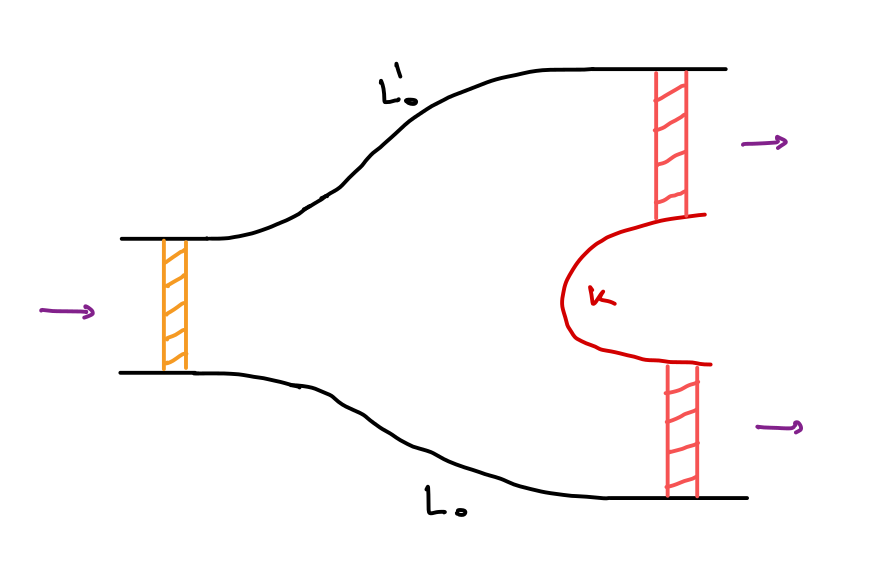
\includegraphics[width=.7\linewidth]{cop1.png}
		\caption{A possible configuration counted for $\Delta_{0|1|0}\colon CF(L_0,L_0')\to CF(L_0,K)\otimes CF(K,L_0').$}
		\label{fig:sfig1}
	\end{subfigure}\hspace{1em}
	\begin{subfigure}{.5\textwidth}
		\centering
		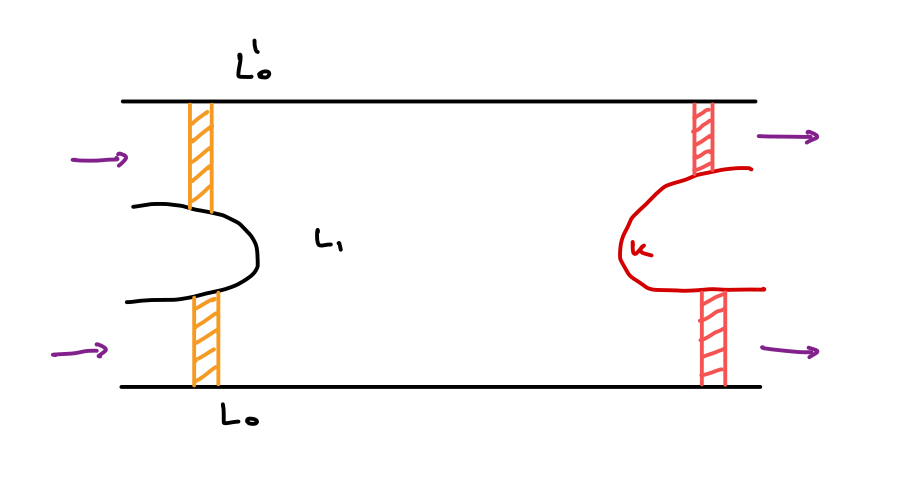
\includegraphics[width=.7\linewidth]{cop2.png}
		\caption{A possible configuration counted for $\Delta_{1|1|0}\colon CF(L_0,L_1)\otimes CF(L_1,L_0')\to CF(L_0,K)\otimes CF(K,L_0').$}
		\label{fig:sfig2}
	\end{subfigure}\hspace{1em}
	\begin{subfigure}{.5\textwidth}
		\centering
		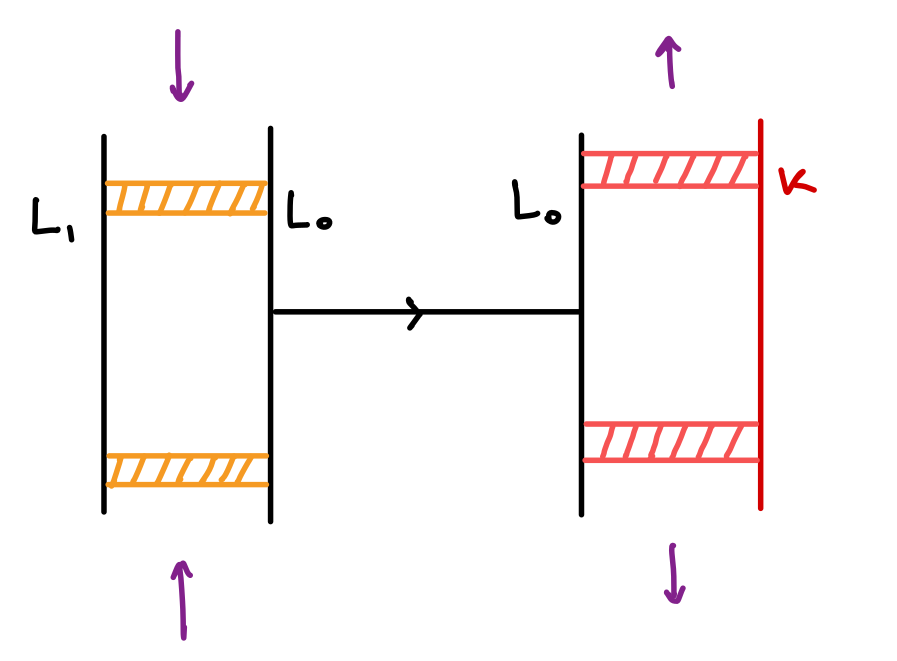
\includegraphics[width=.7\linewidth]{cop3.png}
		\caption{A possible configuration counted for $\Delta_{1|1|0}\colon CF(L_0,L_1)\otimes CF(L_1,L_0)\to CF(L_0,K)\otimes CF(K,L_0).$ The horizontal line segment represents a finite Morse flowline on $L_0$.}
		\label{fig:sfig3}
	\end{subfigure}
	\caption{Examples of configurations contributing to the coproduct $\Delta^{\mathcal{B},K}_q\colon \Delta_{\mathcal{B}_p}\to \mathcal{Y}_{p}^l(K)\otimes \mathcal{Y}_{p}^r(K)$. The colored strips indicate the support of the non-trivial parts of Hamiltonian perturbation data.}
	\label{fig:coproduct}
\end{figure}
\begin{proof}
The construction of $\Delta$ depends on the construction of certain moduli spaces whose definition is 
well understood (see \cite{Ab:geom-crit}, \cite{she:fanofuk}). Therefore, we will only sketch the construction and only emphasize the adjustments required to ensure that $\Delta$ has a controlled shift in action filtration. We sketch in Figure \ref{fig:coproduct} some configurations of clusters contributing to the definition of $\Delta$. 

	

 Let $\epsilon>0$ and fix a regular filtered perturbation datum $p\in \mathcal{P}$ of size $\nu(p)=\epsilon$. $\Delta$ will consists of a family of linear maps $$\Delta_{l|1|r}\colon CF(L_0,\ldots, L_l)\otimes CF(L_l,L_0')\otimes CF(L_0',\ldots, L'_r)\to CF(L_0,K)\otimes CF(K,L'_r)$$ for any $l,r\geq 0$ and any two tuples $\vec{L}=(L_0,\ldots, L_l)$ and $\vec{L'}=(L'_0,\ldots, L'_r)$ of Lagrangians in $\mathcal{B}$, where all the Floer chain complexes are defined with respect to $p$. The source spaces for $\Delta_{l|1|r}$ are parametrized by  moduli spaces of clusters (following the terminology in  Chapter \ref{ch:ffuk}) $\mathcal{R}^{l,r,2}_C(\vec{L},\vec{L'},K)$ labelled by $\vec{L}$, $\vec{L'}$ and $K$ defined as follows:
\begin{enumerate}
	\item We start with the moduli space $\mathcal{R}^{l,r}(\vec{L},\vec{L'},K):=\mathcal{R}^{l+r+3}(\vec{L}\cup\vec{L'}\cup K)$ of disks with $l+r+3$ marked points, labelled by our fixed Lagrangians as follows: we choose a marked point and label by $K$ the first arc going clockwise from this point and then keep on labelling clockwise successive arcs first with $\vec{L}$, and then with $\vec{L'}$.
	\item Over $\mathcal{R}^{l,r}(\vec{L},\vec{L'},K)$ we have a bundle $$\pi^{l,r}(\vec{L},\vec{L'},K)\colon \mathcal{S}^{l,r}(\vec{L},\vec{L'},K)\to \mathcal{R}^{l,r}(\vec{L},\vec{L'},K)$$ such that given $r\in \mathcal{R}^{l,r}(\vec{L},\vec{L'},K)$ its preimage is the standard unit disks with labels and prescribed marked points but with the marked points where two arcs corresponding to geometrically different Lagrangians meet replaced by a puncture.
	\item We endow $\mathcal{R}^{l,r}(\vec{L},\vec{L'},K)$ with strip-like ends in the usual manner: near marked points adjacent to the arc labelled by $K$, we choose positive strip-like ends, while on the remaining $l+r+1$ marked points we choose negative ones (this choice will be required to be consistent with gluing and breaking of disks, as usual).
	\item We consider the compactification $\overline{\mathcal{R}^{l,r}(\vec{L},\vec{L'},K)}$ of $\mathcal{R}^{l,r}(\vec{L},\vec{L'},K)$ which has the structure of a manifold with corners
%\footnote{If the strip-like ends are chosen in a compatible way, which we do, even though we will not go into details here.} 
of dimension $l+r+1$, and add collar neighbourhoods to some boundary components as \cite[p. 14]{Amb:fil-fuk} to get the needed moduli space  $\mathcal{R}_C^{l,r}(\vec{L},\vec{L'},K)$
	\item Over this moduli space we define the bundle $$\pi_C^{l,r}(\vec{L},\vec{L'},K)\colon \mathcal{S}_C^{l,r}(\vec{L},\vec{L'},K)\to \mathcal{R}_C^{l,r}(\vec{L},\vec{L'},K)$$ where fibers are cluster of marked disks with punctures with $l+r+1$ entries and two (adjacent) exits.
\end{enumerate}
Similarly to the case of filtered $A_\infty$-categories (developed in Chapter \ref{ch:ffuk}), there is a space $\mathcal{P}^{\Delta}(p,\mathcal{B},K)$ of universal choices of perturbation data on the family of bundles of clusters $\pi_C^{l,r}(\vec{L},\vec{L'},K)$ (with fixed $K$), and an associated compatibility requirement with the fixed choice of perturbation datum $p\in \mathcal{P}$. 

Given a choice of $q\in \mathcal{P}^{\Delta}(p,\mathcal{B},K)$, of tuples $\vec{L}$ and $\vec{L'}$ as above,
 and of generators $$\gamma_0\otimes \cdots \otimes \gamma_l\otimes \gamma\otimes\gamma'_0\otimes \cdots \otimes \gamma'_r \in CF(L_0,\ldots, L_l)\otimes CF(L_l,L_0')\otimes CF(L_0',\ldots, L'_r)$$ and $$\gamma^+_1\otimes \gamma^+_2\in CF(L_0,K)\otimes CF(K,L'_r)$$ we have the moduli spaces $$\mathcal{M}^{l+r+1}_{\vec{L},\vec{L'},K}(\gamma_0,\ldots, \gamma_l;\gamma;\gamma'_1,\ldots, \gamma_r;\gamma^+_1,\gamma^+_2;q)$$ of Morse-Floer clusters $u$ defined for the perturbation datum $q$, joining such generators. One then defines $\Delta_{l|1|r}$ by counting rigid clusters $u$ in these moduli spaces, weighted by their symplectic area (by multiplication with $T^{\omega(u)}$, with $T$ the Novikov ring variable). Standard compactness and transversality arguments then show that for a generic choice of $q\in \mathcal{P}^{\Delta}(p,\mathcal{B},K)$ these maps fit together into a morphism of $A_\infty$-bimodules $$\Delta\colon \Delta_{\mathcal{B}_p}\to \mathcal{Y}^l_{p}(K)\otimes \mathcal{Y}^r_{p}(K)$$ which, of course, depends on the choice of the perturbation datum $q$. Most importantly, the filtered properties of $\Delta$ strongly depend on the choice of $q$: for an arbitrary choice of $q$ there is no reason to expect that the associated morphism $\Delta$ has a controlled shift in filtration. 
However, the same idea introduced in Chapter \ref{ch:ffuk} for the case of the $\mu_d$-maps can be replicated here to control the shift of the map $\Delta$. 
 %the idea is to choose perturbation data for the source space with one input and two exits that are supported on strip %like ends, and on each strip-like end they restrict to smart monotone homotopies from the Hamiltonian Floer data to %the zero map (and viceversa, depending on the sign of the strip-like end), and then construct perturbation data for %source spaces with more inputs inductively using gluing with lower order ones and ones coming from $p$. 
 Notice that the term $\Delta_{0|1|0}\colon CF(L,L)\to CF(L,K)\otimes CF(K,L)$ counts Floer curves with a Morse input (recall that we defined $CF(L,L)$ using the pearly model) and two Floer outputs (as $K\notin \mathcal B$ by assumption), which do not pose any problem from a filtered point of view. % as no "$s$-dependent" perturbation data are needed.  
On the other hand, we encounter some novel problems relative to the constructions described previously when dealing with two different Lagrangians $L_0\neq L_0' $ and the map $ \Delta_{0|1|0}\colon CF(L_0,L_0')\to CF(L_0,K)\otimes CF(K,L_0')$. In this case, the methods from Chapter \ref{ch:ffuk} give a map of shift $\leq 2\nu(p)-\delta\nu(p)\leq 2\nu(p)$. Since the perturbation data for higher order components $\Delta_{l|1|r}$ of $\Delta$ are constructed --following Chapter \ref{ch:ffuk}-- inductively, this shifts propagates. It is important to remark that given the structure of the moduli spaces defining $\Delta_{l|1|r}$ this shift does not grow proportionally to the order, but remains $\leq 2\nu(p)$. Indeed near corners of $\overline{\mathcal{R}_C^{l,r}(\vec{L},\vec{L'},K)}$, the inductively constructed perturbation data come from gluing of perturbation data associated with configurations with $\leq 3$ marked points, of which at most one is a configuration with one entry and two exit (that is, on which $\Delta_{0|1|0}$ is modeled on) and contributes positively to the curvature (and the contribution is bounded above by $2\nu(p)$ as explained above); all the other configuration involved in the gluing have only one output, and do not contribute to the curvature (see Figure \ref{fig:cop_near_bdry}).
% 
%  and $\Delta_{0|1|1}$. These maps are defined through counts of Floer clusters with domains curves with two entries and two exits. The bound on the curvature terms on these curves equals (up to an arbitrarily small summand due to transversality-related perturbations, see \cite[p. 35]{Amb:fil-fuk}) $$2\nu(p)-2\delta\nu(p)$$ where we recall that $\delta\in \left(\frac 12,1\right)$ is a fixed constant. This is precisely because we have {\em two} exits (the positive $2\nu(p)$ term) and two entries (the negative $2\delta\nu(p)$) term. 
% 
%There is an easy way to address  this issue but the solution restricts the available perturbation choices
% from $\mathcal{P}$ to a subclass $\mathcal{P}(\mathcal{B})\subset \mathcal{P}$ that we now describe.
% Fix $\eta\in \left(0,\frac{2\nu(p)}{2}(1-\delta)\right)$.  The perturbation data $p\in \mathcal{P}(\mathcal{B})$
% is characterized by the following two properties:
% \begin{itemize}
% \item[-] Let $L$ and $L'$ be two distinct Lagrangians in $\lagmon$ such that  $L,L'\in\mathcal{B}$. 
% The  Hamiltonian part of the Floer datum (associated with $p$) satisfies $$\text{image}\left(H_p^{L_0,L_1}\right)\subset \left(\frac{2\nu(p)}{2}(1+\delta)+\eta,\nu(p)\right)$$
% \item[-] For two distinct Lagrangians $L,L'$ such that at least one of them is not  in $\mathcal{B}$ we require $$\text{image}\left(H_p^{L_0,L_1}\right)\subset \left(\delta\nu(p),\frac{2\nu(p)}{2}(1+\delta)-\eta\right).$$ 
% \end{itemize} 
% Such a restriction does not interfere with transversality nor with the filtration properties of the $A_\infty$ multiplication maps. At the same time, for such a choice of perturbation datum $p$,  the curvature term of a Floer cluster contributing to $\Delta_{1|1|0}$ or $\Delta_{0|1|1}$ defined via a perturbation datum $q\in \mathcal{P}^{\Delta}(p,\mathcal{B},K)$  is bounded above by the negative quantity $$(\nu(p)(1+\delta)-\eta)-(\nu(p)(1+\delta)+\eta)=-2\eta.$$ It follows that the components $\Delta_{1|1|0}$ and $\Delta_{0|1|1}$ are filtered maps. The same argument applies for components with more entries and this concludes the sketch of the proof of Proposition \ref{coproductmain}.
\end{proof}
\begin{figure}
	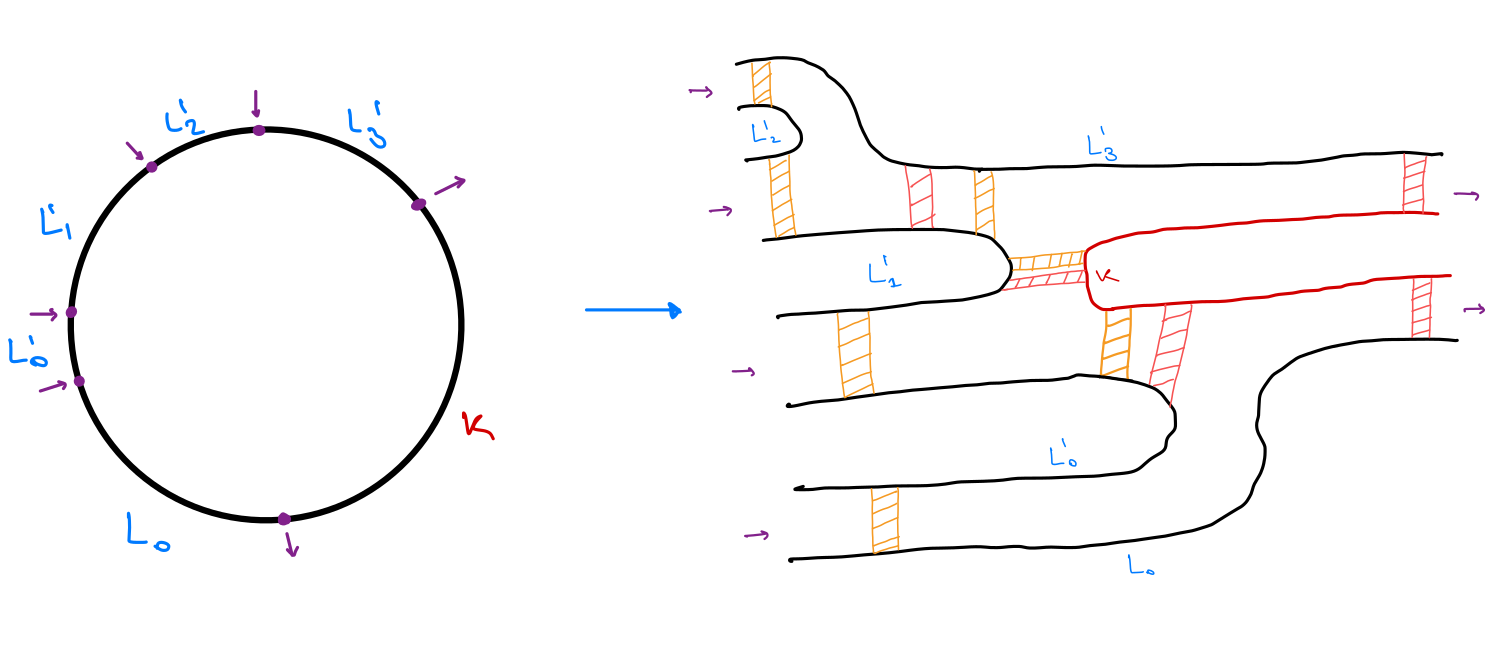
\includegraphics[scale=0.2]{cop_near_bdry.png}
	\centering
	\caption{A curve contributing to $\Delta_{0|1|3}\colon CF(L_0,L_0',L_1',L_2',L_3')\to CF(L_0,K)\otimes CF(K,L_3')$ whose source space lies near a corner point in $\overline{\mathcal{R}_C^{0,3}(\vec{L},\vec{L'},K)}$. The orange strips represent the region where perturbation data contribute negatively to the curvature, while the red strips where it contributes positively. The total curvature is then bounded from above by $2\nu(p)$.} \label{fig:cop_near_bdry}
\end{figure}

\begin{rem}
	It is clear from the proof of Proposition \ref{coproductmain} that the shift $\leq 2\nu(p)$ of the map $\Delta$ is not sharp for our choices of perturbations (indeed, $2\nu(p)-\delta\nu(p)$ can be used as an upper bound). However, we decided to stick to $2\nu(p)$ for notational ease. Since in Theorem \ref{gio:wabomain} we work with a system of $A_\infty$-categories, this difference is irrelevant.
\end{rem}
%======================================
%======================================
%======================================
\subsubsection{Ambient quantum cohomology}\label{AQH} The material briefly recalled here is well-known
(see \cite{she:fanofuk} for a possible reference). 
Let $(X,\omega)$ be a closed and monotone symplectic manifold. We consider a Morse function $f\colon X\to \mathbb{R}$ with a unique maximum $u\in X$ and a Riemannian Metric $g$ on $X$ such that the pair $(f,g)$ is Morse-Smale.  We define the quantum cochain complex $CQ^*(f,g;\Lambda)$ with $\Lambda$ coefficients associated with the pair $(f,g)$ as its Morse cochain complex over $\Lambda$, that is coindexed by the Morse index. The differential $d$ counts negative gradient flow lines connecting critical points with index difference equal to one. In the following, we
will denote $CQ(f , g ; \Lambda)$ by $CQ(X; \Lambda)$ when the specific choice of Morse-Smale data is not important for our discussion. We filter this complex by setting every generator at zero action level and using the standard filtration on $\Lambda$. The homology of this complex is denoted by $QH(X;\Lambda)$ and  is called the quantum cohomology of $X$. Note that neither the vector space nor the persistence structure of $QH(X;\Lambda)$ depends on the choice of the Morse-Smale pair. We endow $\QH(X,\La)$ with the standard $\mathbb{R}/2\mathbb{Z}$ grading, with the Novikov variable having degree $0$.

The vector space $QH(X;\Lambda)$ is endowed with a product which deforms the usual Morse product, denoted by $*$ and called the quantum product. This product is defined at the chain level by counting (and weighting in the Novikov coefficient by the symplectic area of) $J$-holomorphic spheres with three marked points, which  lie in stable and unstable manifolds of perturbations of the Morse function $f^M$, much like in the definition of the $A_\infty$-maps for tuples of identical Lagrangians in the definition of the filtered Fukaya category. The quantum product with the first Chern class $c_1(X)$ defines an endomorphism of $QH(X;\Lambda)$ and hence we have a decomposition $$QH^*(X;\Lambda) = \bigoplus_{\mathbf{d}} QH^*(X;\Lambda)_\mathbf{d}$$ where the index corresponds to eigenvalues $\mathbf{d}\in \Lambda$ of this endomorphism, and $QH(X,\Lambda)_\mathbf{d}$ is the eigenspace associated with the eigenvalue $\mathbf{d}\in \Lambda$. It is well known that the Fukaya category associated with the class $\lagmon$ is non-trivial if and only if $\mathbf{d}$ is an eigenvalue of the map above. Moreover, all the eigenvalues $\mathbf{d}$ in fact lie in $\Lambda_0$.

%======================================
%======================================
%======================================


\subsubsection{The persistence open-closed and closed-open maps}\label{gio:oc}
In this section we first define a persistence version of the open-closed map $OC$ relating Fukaya categories with ambient quantum cohomology. This  follows standard constructions in the subject  (cfr. \cite{Ab:geom-crit, she:fanofuk}) therefore we only give details sufficient to justify the persistence aspects.


Let $\mathcal{B}\subset \lagmon$ be a finite subset. Let $\epsilon>0$ and fix a regular filtered perturbation datum $p\in \mathcal{P}$ of size $\nu(p)=\epsilon$. 

We now outline the construction of the persistence open-closed map 
\begin{equation}\label{eq:oc_map}
OC=OC^\mathcal{B}_p\colon PHH(\mathcal{B}_p)\to QH(X,\Lambda)
\end{equation} where $\mathcal{B}_p$ is the full subcategory of $\fuk(\lagmon;p)$ induced by $\mathcal{B}$, and $PHH(\mathcal{B}_p)$ stands for the Hochschild homology of $\mathcal{B}_p$ with coefficients in the diagonal bimodule of $\mathcal{B}_p$ (see Appendix \ref{app:PHH}). 

\

Recall that $OC$ shifts degree up by $n \mod 2$. At the chain level, $OC$ consists of a family of linear maps $$OC_d\colon CF(L_0,L_1)\otimes \cdots \otimes CF(L_{d-1},L_d)\otimes CF(L_d,L_0)\to CQ(X,\Lambda) $$ for each tuple $\vec{L}=(L_0,\ldots, L_d)$ of Lagrangians in $\mathcal{B}$, where all the Floer chain complexes are defined with respect to the perturbation data $p$. 
The construction of these maps is based on moduli spaces and corresponding choices of perturbation data that follows the scheme used to define the filtered
$A_{\infty}$ operations $\mu_{d}$ in Chapter \ref{ch:ffuk} with a few modifications that we now outline. 

\begin{itemize}
\item[-]The perturbed $J$-holomorphic polygons $u$ used to define $OC_{d}$
only have negative strip-like ends near the punctures (by contrast, in the $\mu_{d}$ case, there is one positive strip-like end).
\item[-]  There is an interior marked point $x_{u}$ in the interior of the domain of $u$. 
\item[-] There is a fixed Morse smale pair $(f^X,g^X)$ on $X$ as in the definition $QH(X,\Lambda)$, and an $\omega$-compatible almost complex structure $J$ on $X$ as needed to define the quantum product on $QH(X,\Lambda)$. The equation satisfied by $u$ is $J$-holomorphic (without Hamiltonian perturbations)
in a small neighbourhood of $x_{u}$.
\item[-]  Given $$\gamma_1\otimes\cdots\otimes \gamma_{d+1}\in CF(L_0,L_1)\otimes \cdots \otimes CF(L_d,L_0)$$ and a critical point $x$ of $f^X$, there are moduli spaces $$\mathcal{M}^{d+1,1}_{\vec{L}}(\gamma_1,\ldots, \gamma_{d+1};x;q)$$ defined just like in the definition
of the $\mu_{d}$'s except that the output condition is replaced by the requirement that $u(x_{u})$ is carried by a trajectory of $-\nabla_{g^{X}}f^{X}$ to $x$.  
\item[-] $OC_{d}$ is defined by counting rigid curves as in the moduli space
above. Of course, these moduli spaces are defined with respect to regular perturbation data that is compatible  in the obvious sense with $p$.
\end{itemize}


\begin{figure}
	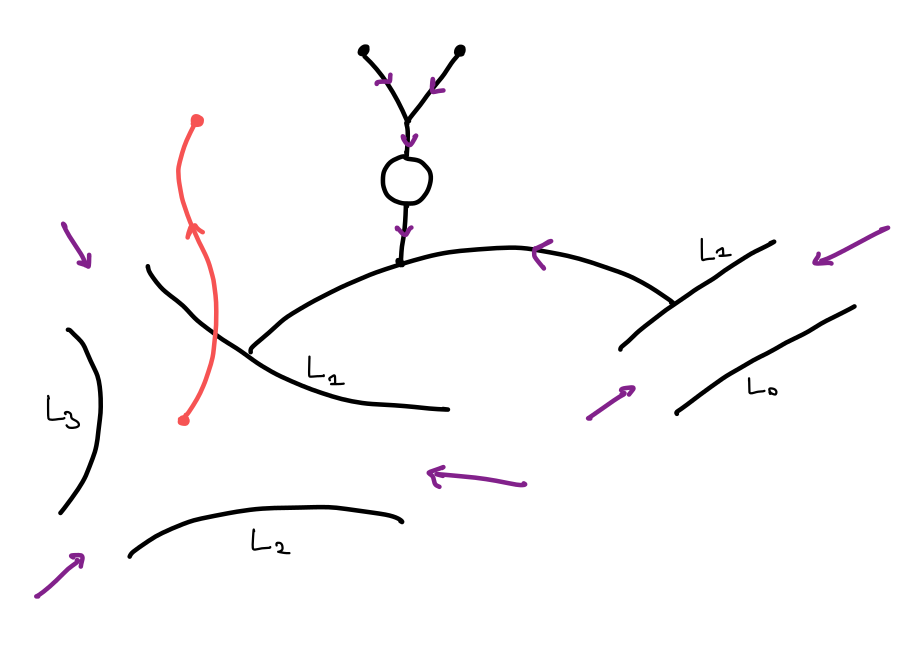
\includegraphics[scale=0.4]{OCfig.png}
	\centering
	\caption{A curve counted in the definition of $OC_7$ for the tuple $\vec{L}=(L_0,L_1,L_1,L_1,L_3,L_2,L_1,L_0)$.} \label{fig:OC}
\end{figure}


%
%At the chain level these maps depend on several choices. The source spaces for $OC_d$ are parametrized by a moduli space of clusters $\mathcal{R}^{d+1,1}_C(\vec{L})$ labelled by $\vec{L}$ defined as follows:
%\begin{enumerate}
%	\item Start with the moduli space $\mathcal{R}^{d+1,1}(\vec{L})$ of disks with $d+1$ boundary marked points and one interior marked point, labelled by our fixed Lagrangians as follows: choose a distinguished marked point and label  the arcs starting from this point, in clockwise direction,  by $L_0$, $L_{1}$ and so forth. 
%	\item Over $\mathcal{R}^{d+1,1}(\vec{L})$ consider a bundle $$\pi^{d+1,1}(\vec{L})\colon \mathcal{S}^{d+1,1}(\vec{L})\to \mathcal{R}^{d+1,1}(\vec{L})$$ such that  $r\in \mathcal{R}^{d+1,1}(\vec{L})$ has as 
%fiber the standard unit disk with one interior marked point and  with boundary punctures replacing the boundary marked points. The arcs on the boundary  remain labeled  as at (1).  
%	\item Endow $\mathcal{R}^{d+1,1}(\vec{L})$ with {\em only} negative strip-like ends near the punctures and with a positive cylindrical end near the interior marked point.
%	\item Consider the  compactification $\overline{\mathcal{R}^{d+1,1}(\vec{L})}$ of $\mathcal{R}^{d+1,1}(\vec{L})$. This has the structure of a manifold with corners of dimension $l+r+1$. We add collar neighbourhoods to some boundary components as \cite[p. 14]{Amb:fil-fuk} to get the moduli space of clusters $\mathcal{R}_C^{d+1,1}(\vec{L})$.
%	\item Define the bundle $$\pi_C^{d+1,1}(\vec{L})\colon \mathcal{S}_C^{d+1,1}(\vec{L})\to \mathcal{R}_C^{d+1,1}(\vec{L})$$ with fibers  cluster of marked disks with punctures with $d+1$ entries and one interior exit.
%\end{enumerate}
%Similarly to the case of the $A_\infty$ multiplication $\mu_{d}$ (Chapter \ref{ch:ffuk}, Chapter \ref{ch:ffuk}) and of the coproduct from \S\ref{gio:coproduct},  there is a space of perturbation choices supported on 
%$\pi_C^{d+1,1}(\vec{L})$ that satisfy a compatibility requirement with the fixed choice of perturbation data $p\in \mathcal{P}$. One novelty here is that we are now dealing with an interior marked point, and we require our perturbations to be such that the Hamiltonian part vanishes on the cylindrical end around this point. Moreover, the almost complex structure is fixed there. 
%Further, the perturbation datum for $\pi_C^{d+1,1}(\vec{L})$ includes the choice of a Morse-Smale pair $(f^X,g^X)$ on $X$ (needed to define $QH(X,\Lambda)$), and of an $\omega$-compatible almost complex structure on $X$ (needed to define the quantum product on $QH(X,\Lambda)$). Let's denote by $\widetilde{\mathcal{P}}^{OC}(p,\mathcal{B})$ the space of such perturbation data compatible with a fixed choice of $p\in \mathcal{P}$. Given a choice of $q\in \widetilde{\mathcal{P}}^{OC}(p,\mathcal{B})$ and a tuple $\vec{L}=(L_0,\ldots, L_d)$ as above and generators $$\gamma_1\otimes\cdots\otimes \gamma_{d+1}\in CF(L_0,L_1)\otimes \cdots \otimes CF(L_d,L_0)$$ and $x\in CQ(X,\Lambda)$ (that is, a critical point of $f^X\colon X\to \mathbb{R}$) we can define moduli spaces $$\mathcal{M}^{d+1,1}_{\vec{L}}(\gamma_1,\ldots, \gamma_{d+1};x;q)$$ of Morse-Floer clusters defined via the perturbation datum $q$, joining such generators. We recall that $x$ is connected to the rest of the cluster via an incoming semi-infinite negative gradient flow trajectory. One then defined the $d$-th component $OC_d$ of the open closed map by counting rigid clusters in these moduli spaces, weighted in the Novikov factor by symplectic area. Again, usual compactness and transversality arguments show that for a generic choice of $q\in \widetilde{\mathcal{P}}^{OC}(p,\mathcal{B})$ the maps $OC_d$ for $d\geq 0$ pack together into a chain map $$OC\colon CC_*(\mathcal{B})\to CQ(X,\Lambda)$$ which depends on the choice of $q$. For general choices of $p$-compatible perturbation $q$, the resulting open-closed map does not preserve filtration. However, we can, again, replicate the idea sketched in Chapter \ref{ch:ffuk} and \ref{gio:coproduct} to get a non-empty subset $\emptyset\neq \mathcal{P}^{OC}(p,\mathcal{B})\subset \widetilde{\mathcal{P}}^{OC}(p,\mathcal{B})$ of regular perturbations such that the associated open-closed map is filtered. 

In this case (because there are no positive-strip-like ends), the arguments showing that the $A_{\infty}$ operations from Chapter \ref{ch:ffuk} are filtered apply directly.  As a result the $OC$ map described above induces  a morphism of persistence modules as in (\ref{eq:oc_map}). Moreover, we also have the following result whose proof is completely analogous to \cite[Corollary 2.11]{she:fanofuk}.
\begin{lem}
	For any $\mathcal{B}$ and any $p\in \mathcal{P}$, $\text{image}(OC^\mathcal{B}_p)\subset QH(X,\Lambda)_\mathbf{d}$, where $\mathbf{d}\in \Lambda_0$ is the parameter prescribing our class of monotone Lagrangians.
\end{lem}

\  

We end this section by briefly recalling from \cite{Bi-Co:rigidity} the definition of the linear part of the closed-open map. Let $p\in \mathcal{P}$ and consider the $\omega$-compatible almost complex structure $J_p^K$-prescribed by $p$ for $CF(K,K)$. Then $CO_p^K\colon CQ(X,\Lambda)\to CF(K,K)$ is defined by counting rigid $J_p^K$-pearly trajectories starting at a critical point of $f_p^X$ and ending at a critical point of $f^K_p$ (see \cite[Figure 3]{Bi-Co:Yasha-fest} with $x=e_K$). Since there is no Hamiltonian perturbation involved, it is straightforward to see that $CO_p^K$ induces a persistence map 

\begin{equation}\label{eq:co_map}
CO=CO_p^K\colon QH(X,\Lambda)\to HF(K,K).
\end{equation} Recall (see \cite[Proposition 2.9]{she:fanofuk}) that $CO$ restricted to $QH(X,\Lambda)_{\mathbf{d}'}$ vanishes unless $\mathbf{d}'=\mathbf{d}$. We recall that $CO$ is unital in the sense that it sends the projection to $QH(X,\Lambda)_{\mathbf{d}}$ of the unit to the unit in $HF(K,K)$.

\begin{rem}
	It is possible to define a version of the richer, more general, (non-linear) closed-open map, that is a persistence map $$CO^\mathcal{B}_p\colon QH^*(X;\Lambda)\to PHH^*(\mathcal{B}_p),$$ where $PHH^*(\mathcal{B}_p)$ denotes the persistence Hochschild cohomology of the $A_\infty$-category $\mathcal{B}_p$, but this goes beyond the scope of this paper.% The first author plans to include a discussion of the retract-approximability criterion using Hochschild cohomology and a persistence version of the Calabi-Yau morphism (see \cite{Gan:thesis, she:bigfuk}) in his Phd thesis.
\end{rem}

%\begin{prop}	Let $p\in \mathcal{P}$. There are persistence maps $$OC^\mathcal{B}_p:PHH_*(\mathcal{B}_p,\mathcal{B}_p)\to QH^{*+n}(X,\Lambda), \quad CO^\mathcal{B}_p\colon QH^*(X,\Lambda)\to PHH^*(\mathcal{B}_p,\mathcal{B}_p)$$ that compute the classical open-closed and closed-open maps \cite{Ab:geom-crit, she:fanofuk} (>>>>).\end{prop}
%We recall from \cite{she:fanofuk} that, in our compact setting, open-closed and closed-open maps are dual to each others.

%======================================
%======================================
%======================================

\subsubsection{Abouzaid retract-approximability criterion for a fixed choice of perturbations}\label{gio:aboappr}
Consider a finite family $\mathcal{B}\subset\lagmon$ of Lagrangians and an element $\mathcal{K}\in \lagmon\setminus \mathcal{B}$. We recall the class $\mathcal{P}(\mathcal{B})\subset\mathcal{P}$ of perturbations adapted to $\mathcal{B}$ defined in \S\ref{gio:coproduct}. Let $p\in \mathcal{P}(\mathcal{B})$. The coproduct $\Delta_p\colon \Delta_{\mathcal{B}_p}\to \mathcal{Y}_{p}^l(K)\otimes \mathcal{Y}_{p}^r(K)$ constructed as in \S\ref{gio:coproduct} (where we often dropped the subscript $p$ from the notation) induces a  filtered chain map, which we still denote by $\Delta_p$, $$\Delta_p\colon CC_*(\mathcal{B}_p)\to \Sigma^{-2\nu(p)}CC_*(\mathcal{B}_p,\mathcal{Y}^l(K)\otimes \mathcal{Y}^r(K))$$ (see \cite[Equation 2.178]{Gan:thesis}) defined by  $$\Delta_p(\gamma_1\otimes \cdots \otimes \gamma_{d+1}) := \sum_{i=0}^{d+1}\sum_{j=i}^{d+1}(\Delta_p)_{d-j|1|i}(\gamma_{j+1},\ldots, \gamma_{d+1},\gamma_1,\ldots,\gamma_i)\otimes \gamma_{i+1}\otimes \cdots \otimes \gamma_j.$$ Consider the filtered chain isomorphism $\varphi: CC_*(\mathcal{B}_p,\mathcal{Y}^l(K)\otimes \mathcal{Y}^r(K))\cong \overline{\mathcal{B}_p}(K,K)$ given by rotating pure tensors once to the left.  It is defined on a pure tensor $$a\otimes b\otimes \gamma_1\otimes \cdots \otimes \gamma_n\in  CC_*(\mathcal{B}_p,\mathcal{Y}^l(K)\otimes \mathcal{Y}^r(K))$$ as $$\varphi(a\otimes b\otimes \gamma_1\otimes \cdots \otimes \gamma_n):= b\otimes \gamma_1\otimes \cdots \otimes \gamma_n\otimes a.$$  In the following we will consider the composition $$(\Sigma^{-2\nu(p)}\varphi)\circ \Delta_p\colon CC_*(\mathcal{B}_p)\to \Sigma^{-2\nu(p)}\overline{\mathcal{B}_p}(K,K),$$ and, by a slight abuse of notation, still denote this by $\Delta_p$.

%\ocnote{Please write what this ``filterered chain isomorphism $\varphi$'' is as it's hard to follow, also write explicitly what is $\Delta_{p}$ in the next diagram - maybe like I did above}.  


\begin{prop}\label{gio:propabo}
	Let $p\in \mathcal{P}$. Then there is a commutative diagram of persistence modules and maps
	\begin{equation}		\label{persistencediagram} \xymatrixcolsep{3pc}
	\xymatrixrowsep{3pc} \xymatrix{PHH(\mathcal{B}_p) \ar[r]^-{\Delta_p}
		\ar[d]_-{OC^\mathcal{B}_p} & \Sigma^{-2\nu(p)} H(\overline{\mathcal{B}_p}(K,K))
		\ar[d]^-{\Sigma^{-2\nu(p)}\mu^{\overline{\mathcal{B}_p}}}\\
		QH(X,\Lambda) \ar[r]^-{\eta_{2\nu(p)} \circ CO^K_p} & \Sigma^{-2\nu(p)}HF(K,K) }
\end{equation}
	where $\eta_{2\nu(p)}\colon HF(K,K)\to \Sigma^{-2\nu(p)}HF(K,K)$ is the standard map induced by the structural maps of the persistence module $HF(K,K)$ as in \cite[Section 2.2.4]{BCZ:tpc}.
\end{prop}

\noindent Consider the measurement $R(-,-)$ introduced in (\ref{eq:en_gap}) 
and denote by $u_\mathbf{d}$ the projection of the unit in $QH(X,\La)$ to $QH(X,\La)_\mathbf{d}$.
\begin{cor}\label{gio:keycor}
	Let $p\in \mathcal{P}$. 
	If $R(u_\mathbf{d},OC^\mathcal{B}_p)\leq \alpha$, then $\lagmon$ is $\frac{\alpha}{2}+\nu(p)$-retract approximable in $PD(\mathcal{A}_p)$ by the family $\mathcal{B}$.
\end{cor}
The proof of the Corollary will make use of the following simple result.
\begin{lem}\label{ezlemma2}
	Let $f\colon V\to W$ be a map of persistence modules and consider $w\in W_r$. Given $\delta>0$ we have $$R(w,f)\leq R(i_{r,r+\delta}(w),\Sigma^{-\delta}f)+\delta.$$ 
\end{lem}
\begin{proof}
	Consider $\Sigma^{-\delta}f\colon \Sigma^{-\delta}V\to \Sigma^{-\delta}W$ and $i^W_{r,r+\delta}(w)\in (\Sigma^{-\delta}W)_r$. Let $s\geq r$ such that there is $v\in (\Sigma^{-\delta}V)_s$ with $(\Sigma^{-\delta}f)_s(v) = i^{\Sigma^{-\delta}W}_{r,s}(i^W_{r,r+\delta}(w))$. Since $i^{\Sigma^{-\delta}W}_{r,s} = i^{W}_{r+\delta,s+\delta}$ and $(\Sigma^{-\delta}V)_s=V_{s+\delta}$ the above is equivalent to $f_{s+\delta}(v) = i^W_{r,s+\delta}(w)$. In particular, $s+\delta\geq R(w,f)$.
\end{proof}
%\begin{proof}
%	Let $v'\in V'_{s'}$ for some $s'\geq {r'}$ such that $f'_{s'}%(v')=i^{W'}_{r',s'}(w')$. Then $$f_{s'}\circ h^V_{s'}(v') = %h^{W}_{s'}\circ f'_{s'}(v') =  h^W_{s'}\circ i^{W'}_{r',s'}(w') %= i^{W}_{r',s'}\circ h^W_{r'}(w') = i^{W}_{r',s'}\circ i^{W}%_{r,s'}(w) = i^{W}_{r,s'}(w)$$ proving the claim.
%\end{proof}
\begin{proof}[Proof of Corollary \ref{gio:keycor}]	
%We return to the proof of the Corollary and a
Assume that $R(u,OC^\mathcal{B}_p)\leq \alpha$. By Lemma \ref{ezlemma}, Proposition \ref{gio:propabo}, Lemma \ref{ezlemma2} and the fact that $CO$ is unital, we directly get $R([e_K],[\mu^{\overline{\mathcal{B}}}])\leq \alpha+\nu(p)$ for all $K\in \lagmon$. Using Proposition \ref{gio:algfilabo} this implies the claim.	
\end{proof}
\begin{proof}[Proof of Proposition \ref{gio:propabo}.]
The proof is essentially a combination of the proofs of Theorem 8.1.1 in \cite{Bi-Co:Yasha-fest} and Lemma 2.15 in \cite{she:fanofuk} while keeping track of the changes in filtration. 

We outline the construction of a chain homotopy $H\colon CC_*(\mathcal{B}_p)\to \Sigma^{-2\nu(p)}CF(K,K)$
that makes  Diagram (\ref{persistencediagram}) commutative. 
Given a tuple $\vec{L}:=(L_0,\ldots, L_d)$ of elements chosen from the family $\mathcal{B}$, we intend to define $$H\colon CF(L_0,\ldots, L_d,L_0)\to \Sigma^{-2\nu(p)}CF(K,K).$$ This again consists of three steps: picking the correct moduli space (this part is already present in the literature);
adjust the spaces of perturbations conveniently so that the construction is compatible with
filtrations (following the methods from Chapter \ref{ch:ffuk}); ensure that the energy bounds are
indeed as required so that the resulting chain homotopy preserves filtrations.




The source spaces for this $H$ are parametrized by a moduli space denoted $\mathcal{R}_C^{d,A}(\vec{L},K)$ (the superscript $A$ indicates that \textit{annuli} appear in the domain) labelled along the boundary by $\vec{L}$ and $K$ and defined as follows:
\begin{enumerate}
	\item We consider the moduli space $\mathcal{R}^{d,A}(\vec{L},K)$ of annular configurations
consisting of an annulus $S^{1}\times [1,\rho]\subset \mathbb{C}$ of unit internal radius and with outside radius $\rho\in (1,\infty)$.  We fix marked points  $z_0=1$, $z_1=-\rho$ as well as $d-1$ other marked points  $z_2,\ldots, z_d$, $|z_{i}|=\rho,\ 1\leq i \leq d$ along the exterior boundary of the annulus, ordered in clockwise direction starting from $z_{1}$.  We  label  the arcs on the exterior circle clockwise by $\vec{L}$ starting from $x_{1}$, and we label the internal circle by $K$.
	\item Over $\mathcal{R}^{d,A}(\vec{L},K)$ we have a bundle $$\pi^{d,A}(\vec{L},K)\colon \mathcal{S}^{d,A}(\vec{L},K)\to \mathcal{R}^{d,A}(\vec{L},K)$$ such that the fiber of a point in
	$\mathcal{R}^{d,A}(\vec{L},K)$  is a boundary-punctured annulus with the interior circle of radius one, the exterior circle of radius some $\rho\in (1,\infty)$ and such that the marked points on the exterior circle that are adjacent to two geometrically distinct Lagrangian labels are replaced with punctures.
	\item We endow $\pi^{d,A}(\vec{L},K)$ with a compatible choice of strip-like ends, all of negative type, associated with each of the punctures at the previous point.
	\item We consider the compactification $\overline{\mathcal{R}_C^{d,A}(\vec{L},K)}$ of $\mathcal{R}_C^{d,A}(\vec{L},K)$. This moduli space of clusters mixes flow lines, disks, and polygons, just as in the definition of the operations $\mu_{d}$ from Chapter \ref{ch:ffuk}, but also has one annular component.  The boundary of $\overline{\mathcal{R}^{d,A}_C(\vec{L},K)}$ in the case $d=1$ is drawn in Figure \ref{fig:deg1}.
	\item There are incidence conditions for each of the marked points and punctures. The punctures correspond to generators of the respective Floer complexes $CF(L_{i},L_{i+1};p)$ (with $p$ the perturbation data); the marked points on the exterior circle (they are so that the adjacent edges have the same label, $L_{j}$, for some $j$) are mapped to critical points of the fixed Morse
	function on $L_{j}$ that is part of $p$; the marked point $z_{o}$ is mapped to a critical
	point of the fixed Morse function on $K$, which is part of the perturbation data $p$. Perturbation data for all of this is picked such that it is compatible with $p\in \mathcal{P}$ and are constructed as in Chapter \ref{ch:ffuk}.
	\end{enumerate}
	\begin{figure}\label{deg1}
		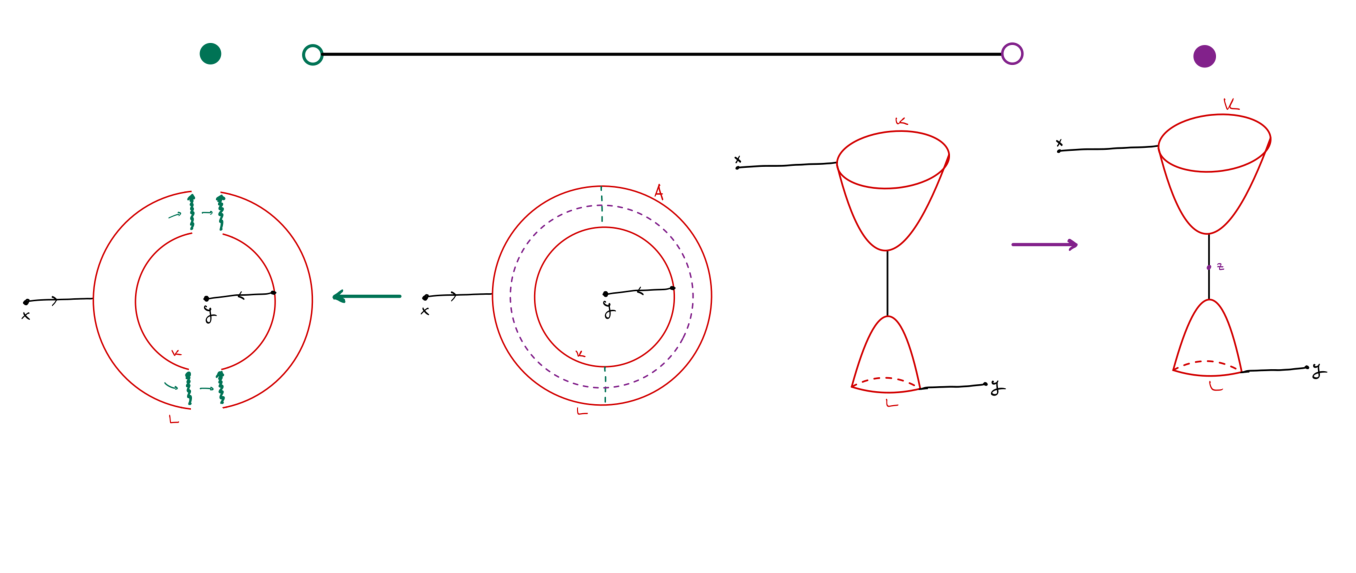
\includegraphics[scale=0.7]{deg1.pdf}
		\centering
		\caption{A schematic description of the interior of $\overline{\mathcal{R}^{1,A}_C(L,K)}$, isomorphic to a closed interval, and the fibers over it. In the middle, given Lagrangians $L$ and $K$ we see configurations contributing to the $y$-summand (where $y\in \text{Crit}(f_K)$) of $H(x)$ (where $x\in \text{Crit}(f_L)$). On the left (green dot) we see the configuration contributing to $\mu_2\circ \Delta$, while on the right (purple dot) a configuration contributing to $OC\circ CO$ (breaking at a critical point $z$ of $f_X$).} \label{fig:deg1}
	\end{figure}

The construction sketched above appeared before in the literature -  see \cite{she:fanofuk} as well as \cite{Bi-Co:Yasha-fest} - and the structure of the compactification $\overline{\mathcal{R}_C^{d,A}(\vec{L},K)}$ implies that it is a chain homotopy as desired. From the point of view of the current 
paper the only additional point of interest is that no further modifications are needed to ensure
that this homotopy is filtration preserving as a map to $\Sigma^{-2\nu(p)}CF(K,K)$ (that is, it shifts filtration by $\leq 2\nu(p)$ as a map to $CF(K,K)$). 
%because all strip-like ends are negative in type and thus the usual energy estimates continue to apply, as in Chapter \ref{ch:ffuk}.

	
%	We define the DMS compactification $\overline{\mathcal{R}^{d,A}(\vec{L},K)}$ of $\mathcal{R}^{d,A}(\vec{L},K)$, which has the structure of a manifold with corners of dimension \TBD and add a collar neighbourhood to some boundary components as in \cite[p. 14]{Amb:fil-fuk} (plus, to the boundary component coming from $\rho \to \infty)$, see Figure \ref{fig:deg1}) to get the needed moduli space of clusters $\mathcal{R}_C^{d,A}(\vec{L},K)$, over which we define the bundle $$\pi_C^{d,A}(\vec{L},K)\colon \mathcal{S}_C^{d,A}(\vec{L},K)\to \mathcal{R}_C^{d,A}(\vec{L},K)$$ where fibers are cluster with punctures with $d$ entries and one exit in the annulus.
%	\item We define the DMS compactification $\overline{\mathcal{R}_C^{d,A}(\vec{L},K)}$ of $\mathcal{R}_C^{d,A}(\vec{L},K)$, which inherits the properties of $\overline{\mathcal{R}^{d,A}(\vec{L},K)}$ directly. The boundary of $\overline{\mathcal{R}^{d,A}_C(\vec{L},K)}$ in the case $d=1$ is drawn in Figure \ref{fig:deg1} (see also footnote \ref{footnote1}).
%	\end{enumerate}
%	\begin{figure}\label{deg1}
%		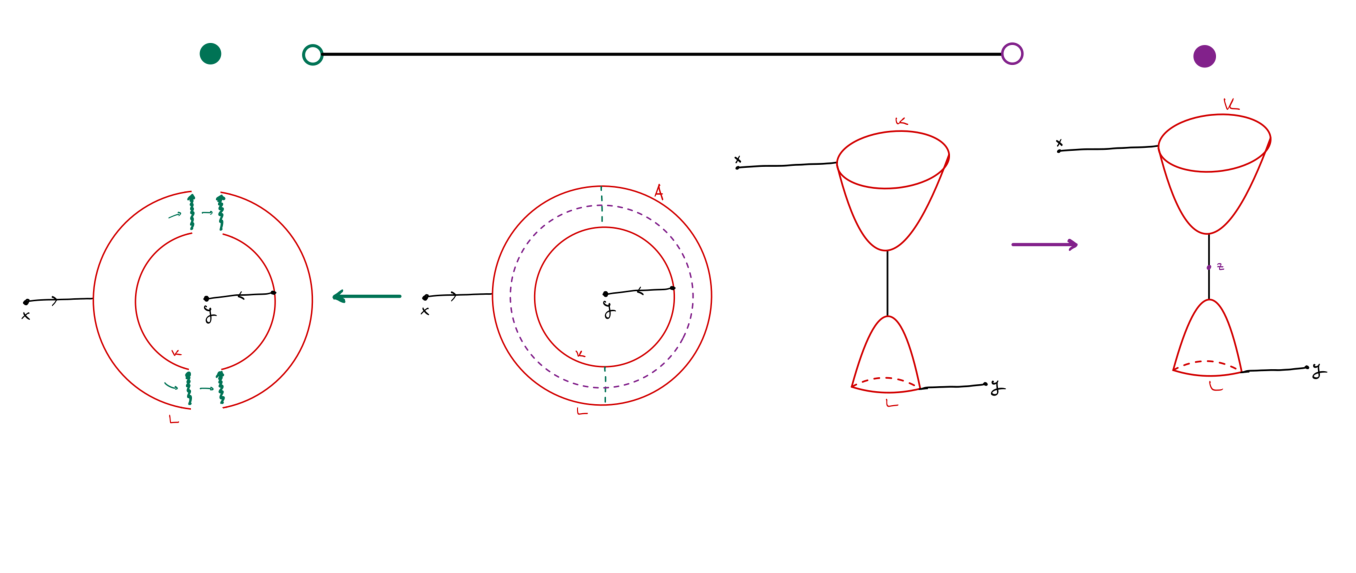
\includegraphics[scale=0.7]{deg1.pdf}
%		\centering
%		\caption{A schematic description of the interior of $\overline{\mathcal{R}^{1,A}_C(L,K)}$, isomorphic to a closed interal, and the fibers over it. In the middle, given Lagrangians $L$ and $K$ we see configurations contributing to the $y$-summand (where $y\in \text{Crit}(f_K)$) of $H(x)$ (where $x\in \text{Crit}(f_L)$). On the left (green dot) we see the configuration contributing to $\mu_2\circ \Delta$, while on the right (purple dot) a configuration contributing to $OC\circ CO$ (breaking at a critical point $z$ of $f_X$).} \label{fig:deg1}
%	\end{figure}
%	
%	
%There is a concept of universal choice of perturbation data on the families $\pi_C^{d,A}(\vec{L},K)$ with varying $\vec{L}$ in $\mathcal{B}$ and fixed $K$, and an associated compatibility requirement with the fixed choice of perturbation datum $p\in \mathcal{P}(\mathcal{B})$ as well as with the choices of elements in $q_\Delta\mathcal{P}(p,\mathcal{B},K)$ and $q_{OC}\mathcal{P}^{OC}(p,\mathcal{B})$. Using the same receipt outlined in the previous section one can define a non-empty class of perturbation data $\mathcal{P}^H(p,q_\Delta,q_{OC})$ such that $H\colon CC_*(\mathcal{B}_p)\to CF(K,K)$ is a filtered chain homotopy\footnote{Note that the boundary $\partial \overline{\mathcal{R}_C^{d,A}(\vec{L},K)}$ of the moduli space of source spaces for $H$ decomposes as the union of terms like $$\bigcup_{d_0\geq 0, \ d_1\geq 2: \ d_0+d_1= =d+1}\bigcup_{\vec{L_0},\vec{L_1}}\mathcal{R}_C^{d_0}(\vec{L_0},K)\times \mathcal{R}^{d_1}(\vec{L_1}\cup K)$$ parametrizing the composition $\mu^{\mathcal{B},K}\circ \Delta^{\mathcal{B},K}$, like $\mathcal{R}^{d,1}_C(\vec{L})\times \mathcal{P}_{CO}(K)$, parametrizing the composition $CO^K\circ OC^\mathcal{B}$ and like $$\mathcal{R}^{d_0}_C(\vec{L_0})\times \mathcal{R}^{d_1,A}_C(\vec{L_1},K)$$ parametrizing the various summands in $H\circ d_{CC}$, where $d_{CC}$ is the Hochschild differential.\label{footnote1}
%} between $CO_p^K\circ OC_{q_{OC}}^\mathcal{B}$ and $\mu^{\mathcal{B},K}_p\circ \Delta^\mathcal{B}_q$. To control the filtration we do not need to impose any new restrictions on the choice of perturbations, since configurations contributing to $H$ have a unique exit, which is of Morse type.
\end{proof}





\begin{rem}
	a. The statement of Proposition  \ref{gio:propabo} contains an intrinsic limitation in the 
	sense  that for a fixed perturbation $p$ it allows to discuss retract-approximability with accuracy bounded below by a constant times $\nu(p)$. Gaining adequate control on the structures associated with a $p$ that varies so that the accuracy level gets below some fixed $\epsilon$ was the main motivation behind the notion of systems of categories with increasing accuracy in \S\ref{s:sys-tpc}. 
	
	b. We could refine the statement of Proposition \ref{gio:propabo} and avoid the shift $\Sigma^{-2\nu(p)}$ in the bottom right of Diagram (\ref{persistencediagram}). This can be done by choosing more elaborate perturbation data for the maps appearing in the diagram. This would have the result of allowing for a slightly better approximation accuracy given a fixed perturbation datum $p$, but the remark above would continue to apply.
	
	b. Note that when $\mathcal{B}$ consists of a single Lagrangian $L$, then $R(u_\mathbf{d}, OC^\mathcal{B}_p)\leq \alpha$ implies that $\lagmon$ is $\frac{\alpha}{2}$-retract approximated in $PD(\mathcal{A}_p)$ by the family $\mathcal{B}$. That is, there is no $\nu(p)$ term appearing in this case, in contrast to the general statement in Corollary \ref{gio:keycor}. The reason is that, in this case, the map $\Delta$ is filtered (see Proposition \ref{coproductmain}); the proof uses a version of Proposition \ref{gio:aboappr} where no shift functor $\Sigma^{-2\nu(p)}$ appears. The only place where this refinement will be used is Proposition \ref{singlelagsphere}.
\end{rem}
	
	
\subsubsection{Colimit of open-closed maps}

In this section we prove that the open-closed map behaves well with respect to continuation functors and define
the colimit open-closed map that appears in the statement of Theorem \ref{gio:wabomain}.


Consider the system $$\widehat{\fuk}(\lagmon)= \left\{\left\{\fuk(\lagmon;p)\right\}_{p\in \mathcal{P}}, \left\{\mathcal{H}_{p,q},\mathcal{H}_{q,p}\right\}_{p\preceq q}\right\}$$ of filtered Fukaya categories associated with $\lagmon$.his is in fact a homotopy system in the sense of \S\ref{sbsb:homotopy-sys}.
As a result of that, via Proposition \ref{p:homotopy-HH}, we get a directed system $$\left\{\left\{PHH(\fuk(\lagmon;p))\right\}_{p\in \mathcal{P}}, \left\{\mathcal{H}_{p,q}^{PHH}\right\}_{p\preceq q}\right\} $$ of persistence modules, where $\mathcal{H}_{p,q}^{PHH}$ is the persistence map induced in persistence Hochschild homology by the (family of) continuation functors $\mathcal{H}_{p,q}$ ($\mathcal{H}_{p,q}^{PHH}$ is uniquely defined by Proposition \ref{p:homotopy-HH}). In particular, the colimit $$PHH(\widehat{\fuk}):=\colim_{p\in \mathcal{{P}}}PHH(\fuk(\lagmon;p))$$ is well-defined and a persistence module, as explained in \S\ref{sb:sys-inv}. Moreover, since the system $\widehat{\fuk}(\lagmon)$ has, in particular, a fixed full base of objects (see \S\ref{sbsb:sys-base}), the following is true: given a subfamily $\mathcal{B}\subset \lagmon$ we get a colimit $$PHH(\widehat{\mathcal{B}}):=\colim_{p\in \mathcal{P}}PHH(\mathcal{B}_p)$$ where $\mathcal{B}_p$ is the full $A_\infty$-subcategory of $\fuk(\lagmon;p)$ induced by $\mathcal{B}$ and $\widehat{\mathcal{B}}$ is the subsystem of $A_\infty$-categories of $\widehat{\fuk}$ induced by $\{\mathcal{B}_p\}_{p\in \mathcal{P}}$.\\

For any $N\geq 1$, we denote by $F^{N}PHH(\mathcal{B}_p)$ the persistence homology of $F^{N}CC(\mathcal{B})$, that is, the $N$-th level in the length filtration of the Hochschild chain complex (see \S\ref{app:PHH}). \\ 
Let $p\preceq q$ and consider the continuation $A_\infty$-functor $\mathcal{H}_{q,p}\colon \mathcal{B}_q\to \mathcal{B}_p$ restricted to $\mathcal{B}_q$. We recall (see Chapter \ref{ch:ffuk}) that these functors have linear deviation rate $\leq 2(\nu(p)-\nu(q))$. We write $s(q,p):= 2(\nu(p)-\nu(q))$. In particular, $\mathcal{H}_{q,p}$ does \textit{not} induce a map in persistence Hochschild homology, as the shift in filtration at the chain level blows up as $N\to \infty$. To overcome this problem, we use the length filtration on $CC(\mathcal{B}_q)$. Note that, at the chain level, $\mathcal{H}_{q,p}$ induces for any $N\geq 1$ a chain map $F^NCC(\mathcal{B}_q)\to F^NCC(\mathcal{B}_q)$ of shift $\leq Ns(q,p)$. In particular, by precomposing and postcomposing with structural maps $\eta$ associated with the shift functor , $\mathcal{H}_{q,p}$ induces a persistence map $$\mathcal{H}_{q,p}^{F^NPHH}\colon \Sigma^{-2N\nu(q)}F^NPHH(\mathcal{B}_q)\to \Sigma^{-2N\nu(p)}F^NPHH(\mathcal{B}_p).$$
The next lemma lemma follows directly from the properties of the continuation functors.
\begin{lem}\label{gio:homcont}
	Let $p\in \mathcal{P}$. The family $$\left\{\mathcal{H}_{q,p}^{F^NPHH}\colon \Sigma^{-2N\nu(q)}F^NPHH(\mathcal{B}_q)\to \Sigma^{-2N\nu(p)}F^NPHH(\mathcal{B}_p)\right\}_{q\in \mathcal{P}, \ p\preceq q}$$ defines a homomorphism of directed systems of persistence modules.
	%By the properties of continuation functors and the definition of the colimit persistence module $PHH(\widehat{\mathcal{B}})$, t
	%In particular, the map $\widehat{OC}^\mathcal{B}$ is well-defined and the maps $\mathcal{H}_{q,p}^{F^NPHH}$ induce a persistence map  $$H^{F^NPHH}_{\infty,p}\colon \Sigma^{-2N\nu(p)}F^NPHH(\widehat{\mathcal{B}})\to F^NPHH(\mathcal{B}_p)$$ for all $p\in \mathcal{P}$. Moreover, the persistence diagram 
	
\end{lem}

Exploiting again the fact that the length filtration is preserved by maps induced on Hochschild chains by $A_\infty$-functors, we define $$F^NPHH(\widehat{\mathcal{B}}):=\colim_{p\in \mathcal{P}}F^NPHH(\mathcal{B}_p)$$ for any $N\geq 1$. 

As a result of Lemma \ref{gio:homcont} and of the fact that $\nu(q)\to 0$ as $q\to \infty$, we get a unique map $$H^{F^NPHH}_{\infty,p}\colon F^NPHH(\widehat{\mathcal{B}})\to \Sigma^{-2N\nu(p)}F^NPHH(\mathcal{B}_p)$$ for any $p\in \mathcal{P}$, such that the diagram 
\begin{equation}		\label{gio:colimitcont} \xymatrixcolsep{3pc}
	\xymatrixrowsep{3pc} \xymatrix{\Sigma^{-2N\nu(q)}PHH(\mathcal{B}_q) \ar[rr]%^-{\Delta_p}
		\ar[dr]_-{\mathcal{H}^{F^NPHH}_{q,p}} & & F^NPHH(\widehat{\mathcal{B}})
		\ar[dl]^-{\mathcal{H}^{F^NPHH}_{\infty,p}}\\
		& \Sigma^{-2N\nu(p)}F^NPHH(\mathcal{B}_p)& }
\end{equation}
commutes for all $q\in \mathcal{P}$ with $p\preceq q$.

So far, what we proved are intrinsic properties of homotopy systems, with no geometric considerations. We now move to geometry and bring in the open-closed maps.

We consider the quantum cohomology $QH(X,\Lambda)$ as a trivial directed system of persistence modules parametrized by $\mathcal{P}$.
\begin{lem}\label{gio:homoc}
	The family of persistence maps $$\left\{OC^\mathcal{B}_p\colon PHH(\mathcal{B}_p)\to QH(X,\Lambda)\right\}_{p\in \mathcal{P}}$$ defines a homomorphism of directed systems of persistence modules. 
\end{lem}
\begin{proof}
	To show that $\{OC^\mathcal{B}_p\}_p$ is a homomorphism of directed systems, we have to prove that $OC^\mathcal{B}_q\circ \mathcal{H}^{PHH}_{p,q}=OC^\mathcal{B}_p$. To this aim, one defines a chain homotopy between the two maps at the chain level, which are filtered chain maps, and shows that it is filtered. This is very similar to the proof of Proposition \ref{gio:propabo} and is omitted here.
\end{proof}

%In Lemma \ref{gio:occont} below we prove that That is, we prove that $$OC^\mathcal{B}_q\circ \mathcal{H}_{p,q}^{PHH} = OC^\mathcal{B}_p$$ for all $p\preceq q$. %In particular, if $i_\infty\circ OC^\mathcal{B}_p$ hits the unit for some $p\in \mathcal{P}$, then the same holds for all other $q\in \mathcal{P}$.
As a result of Lemma \ref{gio:homoc}, we obtain a unique persistence morphism $$\widehat{OC}^\mathcal{B}:=\colim_{p\in \mathcal{P}}OC^\mathcal{B}_p\colon PHH(\widehat{\mathcal{B}})\to QH(X,\Lambda)$$ such that the diagram 
\begin{equation}		\label{gio:colimitoc} \xymatrixcolsep{3pc}
	\xymatrixrowsep{3pc} \xymatrix{PHH(\mathcal{B}_p) \ar[rr]%^-{\Delta_p}
		\ar[dr]_-{OC^\mathcal{B}_p} & & PHH(\widehat{\mathcal{B}})
		\ar[dl]^-{\widehat{OC}^\mathcal{B}}\\
		& QH(X,\Lambda)& }
\end{equation}
commutes for all $p\in \mathcal{P}$. The morphism $\widehat{OC}^\mathcal{B}$ is called the \textit{colimit open-closed map} for $\mathcal{B}$ and is the persistence map appearing in the statement of Theorem \ref{gio:wabomain}.\\

In fact, we will prove more. 


\begin{lem}
	Let $p\in \mathcal{P}$. The persistence diagram \begin{equation}		\label{gio:colimitoc2} \xymatrixcolsep{3pc}
		\xymatrixrowsep{3pc} \xymatrix{\Sigma^{-2N\nu(p)}F^NPHH(\mathcal{B}_p) %^-{\Delta_p}
			\ar[d]_-{\Sigma^{-2N\nu(p)}OC^\mathcal{B}_p}  & &F^NPHH(\widehat{\mathcal{B}}) \ar[ll]^-{\Sigma^{-2N\nu(p)}\mathcal{H}^{F^NPHH}_{\infty,p}}
			\ar[d]^-{\widehat{OC}^\mathcal{B}}\\
			\Sigma^{-2N\nu(p)}QH(X,\Lambda) & & QH(X,\Lambda) \ar[ll] }
	\end{equation} commutes, where the bottom map is induced by the structural maps of the persistence module $QH(X,\Lambda)$.
\end{lem}
\begin{proof}
	Let $p,q$ in $\mathcal{P}$ such that $p\preceq q$. Consider the persistence diagram
	\begin{equation}		\label{gio:colimitoc3} \xymatrixcolsep{3pc}
		\xymatrixrowsep{3pc} \xymatrix{\Sigma^{-2N\nu(p)}F^NPHH(\mathcal{B}_p) %^-{\Delta_p}
			\ar[d]_-{OC^\mathcal{B}_p}  & & F^NPHH(\mathcal{B}_q) \ar[ll]^-{\mathcal{H}^{F^NPHH}_{q,p}}
			\ar[d]^-{OC^\mathcal{B}_q}\\
			\Sigma^{-2N\nu(p)}QH(X,\Lambda) & & QH(X,\Lambda) \ar[ll] }
	\end{equation}
	This diagram commutes, and the proof goes along the same lines as the proof of Lemma \ref{gio:homoc}, with the slight complication that one has to keep track of the shift in filtration. For varying $q$ such that $p \preceq q$, the above diagram induce a commutative diagram of direct systems of persistence modules. Note that the colimit of $\Sigma^{Ns(q,p)}QH(X,\Lambda)$ over this family is equal to $\Sigma^{-2N\nu(p)}QH(X,\Lambda)$. This proves the claim.
\end{proof}

\subsubsection{Proof of Theorem \ref{gio:wabomain}}\label{subsec:proof_split_app}

It is known that the infinity-level open closed map provides an isomorphism $PHH^\infty(\mathcal{B}_p)\cong QH^\infty(X,\Lambda)$ as vector spaces \cite{Gan:thesis}, and that the unit $u\in QH^0(X,\Lambda)$ persists to $QH^\infty(X,\Lambda)$. Any element in $PHH^\infty(\mathcal{B}_p)$ can be represented by a Hochschild chain of length $\leq N_p$ for some $N_p\geq 0$. Moreover, we can choose $N_p$ such that the spectral invariants of $F^{N_p}PHH(\mathcal{B}_p)$ are optimal, i.e. they agree with those of $PHH(\mathcal{B}_p)$ for for the homology classes that persist to infinity in both persistence modules. We claim that $N_p$ is independent of $p\in \mathcal{P}$. This follows from the following fact: by forgetting filtrations, the functors $\mathcal{H}_{q,p}$ induce a unique map $PHH^\infty(\mathcal{B}_q) \to PHH^\infty(\mathcal{B}_p)$ which is an isomorphism  (since, forgetting filtrations, continuation funtors are quasi-equivalence of $A_\infty$-categories) and, hence, preserve the length filtration (note that, of course, all of this holds for the maps induced by $\mathcal{H}_{p,q}$ on $PHH^\infty$). We write $N_\mathcal{B}:=N_p$.

At this point, the proof of Theorem \ref{gio:wabomain} becomes a matter of book-keeping.

	Let $\mathcal{F}^\epsilon\subset \lagmon$ as in the statement. We work with the notation above in the case $\mathcal{B}=\mathcal{F}^\epsilon$. Consider the constant $N_{\mathcal{F}^\epsilon}$ introduced above. Let now $a\in PHH^\epsilon(\widehat{\mathcal{F}^\epsilon})$ be such that $\widehat{OC}(a)=i_{o,\epsilon}(u_\mathbf{d})$, where $u_\mathbf{d}\in QH^0(X,\Lambda)_\mathbf{d}$ is the projection of the cohomological unit in $QH(X,\Lambda)$. From the above it follows that $a$ can be seen as an element in $F^{N_{\mathcal{F}^\epsilon}}PHH(\widehat{\mathcal{F}^\epsilon})$. From this and the commutativity of Diagram (\ref{gio:colimitoc2}) we get $$R(u, OC^{\mathcal{F}^\epsilon}_p)\leq \epsilon+2N_{\mathcal{F}^\epsilon}\nu(p)$$ for all $p\in \mathcal{P}$. Using Proposition \ref{gio:propabo}, we conclude that $\lagmon$ is $\frac{\epsilon}{2}$-retract approximable by $\mathcal{F}^\epsilon$ in the system $\widehat{\fuk}(\lagmon)$ in the sense of Definition \ref{d:approx-sys-ret}. \qed




\begin{rem}
%	a. \TBD The constant $N_{\mathcal{F}^\epsilon}$ appearing in the proof of Theorem \ref{gio:wabomain} depends on the family $\mathcal{F}_\epsilon$, but not really on $\epsilon$: if $\mathcal{F}\subset \lagmon$ is a family such that for all $\epsilon>0$ there is a \textit{finite} subfamily $\mathcal{F}_\epsilon$ satisfying the assumptions of Theorem \ref{gio:wabomain}, then $\mathcal{F}$ approximates $\lagmon$ in $\widehat{\fuk}(\lagmon)$. Indeed, the constant $N_{\mathcal{F}_\epsilon}$ is guaranteed not to explode if the add "useless" (in the sense of $\epsilon$-approximation) Lagrangians to the family $\mathcal{F}_\epsilon$ as $\epsilon\to 0$.
%	\\
%	b. 
	The complex formalism in the proof of Theorem \ref{gio:wabomain} is due to the lack of a concept of colimit of homotopy system of filtered $A_\infty$-categories. Indeed, the open-closed map appearing in the statement of Theorem \ref{gio:wabomain} should be thought as the open-closed map associated with a limit Fukaya category (see the discussion at the beginning of \S\ref{sb:sys-inv}).
\end{rem}








%	In this section we prove that the open-closed map behaves well with respect to continuation functors and prove Theorem \ref{gio:wabomain}.
%	\begin{rem}
%		The complications in the proof of Theorem \ref{gio:wabomain} are due to the lack of a concept of colimit of homotopy system of filtered $A_\infty$-categories. Indeed, the open-closed map appearing in the statement of Theorem \ref{gio:wabomain} should be tought as the open-closed map associated with a limit Fukaya category.
%	\end{rem}
%	\newpage
%	
	
	%=======================================
	%=======================================
	%=======================================
	
	\subsection{Proof of Corollary \ref{S2T2}}\label{gio:proofS2T2}
	% !TEX root = approx8.tex


	We split the proofs of the two geometric situations into subsections. The basic idea is the same: cut the ambient manifold into more and more equally spaced straight slices. We will keep on writing Fukaya categories as $\mathcal{A}_p$ and systems of Fukaya categories as $\widehat{\mathcal{A}}$ as indicated at the beginning of Section \ref{sec:split-app}.
\subsubsection{Approximability of equators on the $2$-sphere} In what follows we will refer to a closed monotone Lagrangian $L\subset S^2$ as an "equator". Note that these Lagrangians are precisely the embedded curves in $S^2$ which separate it into two domeains of equal area.

The first Chern class of $S^2$ vanishes in $H^2(S^2;\mathbb{Z}_2)$, so the eigenspace of the quantum homology $QH(S^2,\Lambda)$ associated to the zero eigenvalue is the whole space. \\ In this subsection, we will only consider (without loss of generality) perturbation data $p\in \mathcal{P}$ satisfying the following two conditions:
\begin{enumerate}
	\item Let $L\in \lag^{\text{(mon,} \mathbf{0} \text{)}}(S^2)$ be an equator on $S^2$ and consider the Morse function $f^L_p\colon L\to \mathbb{R}$ in the $p$-Floer datum of $L$. We assume that $f^L_p$ has a unique maximum $e_L\in L$ and a unique minimum $\text{pt}_L\in L$. We will always assume that both $e_L$ and $\text{pt}_L$ are neither the north nor south poles of $S^2$.
	\item Consider the Morse function $f^{S^2}_p\colon S^2\to \mathbb R$ in the $p$-Floer datum for $S^2$. We assume that $f^{S^2}_p$ has a unique maximum $u_{S^2}\in S^2$ and a unique minimum $\text{pt}_{S^2}\in S^2$ and no other critical points. We further assume that both $u_{S^2}$ and $\text{pt}_{S^2}$ differ from both the north and south poles of $S^2$, 
\end{enumerate}
We will abuse notation and write this "restriction" of $\mathcal{P}$ again as $\mathcal{P}$ and consider the homotopy system of $A_\infty$-categories $\widehat{\mathcal{A}}= \widehat{\fuk}(\lag^{\text{(mon,} \mathbf{0} \text{)}}(S^2))$ as parametrized by this restricted $\mathcal{P}$.
\begin{prop}\label{singlelagsphere}
	Let $L\in \lag^{\text{(mon,} \mathbf{0} \text{)}}(S^2)$ be an equator on $S^2$. Then $\lag^{\text{(mon,} \mathbf{0} \text{)}}(S^2)$ is $\frac{1}{4}$-retract approximable by $L$.
	%for any perturbation datum $p\in E^{sg}$, the open closed-map $OC_p^L\colon HH(L,L)\to QH(S^2)$ satisfies $R(u_{S^2},OC_p^L)\leq \frac{1}{2$}$. {\color{orange} Maybe write it as "Then, for any perturbation datum $p\in E^\mu$ we have $$R(u,OC_p^L)=\frac{1}{2}.$$}
\end{prop}

\begin{proof}
	%We assume that the Morse function $f_L$ associated to the Floer datum of $p$ on $L$ is the height function. Denote by $e_L$ the maximum of $f_L$ and by $\text{pt}_L$ its minumum. Then $CF(L,L)= \Lambda\cdot e_L\oplus \Lambda\cdot \text{pt}_L$. As above, we will work with the height function $f_{S^2}$ on the sphere to define quantum homology, which has a unique maximum $u_{S^2}$ and a unique minumim $\text{pt}_{S^2}$. In particular $CQ(M) = \Lambda\cdot u_{S^2}\oplus \text{pt}_{S^2}$.\\
	%Consider the length filtration $(F^NCC_*(L,L))$ on the Hochschild chain complex as introduced in Section \ref{persistencehochschild}, and the restristion $F^1OC_p^L$ of the chain-level open closed map to $F^1CC_*(L,L)$.
	Let $p\in \mathcal{P}$. It is easy to see
	%that $$OC_p^L(\text{pt}_L\otimes e_L) = OC_p^L(e_L\otimes \text{pt}_L) = OC_p^L(e_L\otimes e_L) = 0 $$
	that at the chain level we have $$OC_p^L(\text{pt}_L\otimes \text{pt}_L) = T^{\frac{1}{2}}u_{S^2}.$$ Moreover, since $d_{CC}$ is cyclic, $\text{pt}_L\otimes \text{pt}_L$ is a cycle in $CC_*(L,L)$. Note that the persistence Hochschild homology $PHH_*(L_p)$ does not depend on $p\in \mathcal{P}$. The claim then follows by Theorem \ref{gio:wabomain}.
	%All of the listed elements in $F^1CC(L,L)$ are cycles as $d_{CC}$ is cyclic. The reason behind the fact that there is no $\text{pt}_{S^2}$ contribution in $OC_p^L(\text{pt}_L\otimes \text{pt}_L)$ has to do with transversality of pearly trajectories; for the same reason that there is no ${\text{pt}}_{S^2}$ contribution in the quantum product ${\text{pt}}_{S^2}*{\text{pt}}_{S^2}= Tu_{S^2}$. {\color{orange} see appendix B for the converse.}
\end{proof}
\begin{rem}
a. We actually proved that for a single equator the constant $\delta>0$ appearing in Definition \ref{d:approx-sys-ret} can be taken to be arbitrarily big. This is due to the fact that for the self-Floer homology of $L$ we do not need any Hamiltonian perturbation.

b. The linear component $ HF(L,L)\to QH(S^2)$ of the open-closed map does not hit the unit in our setting: indeed $OC(e_L)=0$ by a degree argument while $OC(\text{pt}_L) = \text{pt}_{S^2}+T^{\frac{1}{2}}u_{S^2}$. Note however, that if we would have worked with coefficients in the Novikov field over the real numbers, the situation would have been different, as $T^{-1\frac{1}{2}}\text{pt}_{S^2}+u_{S^2}$ is the projection of the unit in the zero eigensummand of quantum homology of $\mathcal{C}P^1$ over this coefficient field.\\ Note that as $\text{pt}_{S^2}+T^{\frac{1}{2}}u_{S^2}$ and $u_{S^2}$ are non-homologous cycles in $CQ(S^2)$, it follows that $[\text{pt}_{L}]$ and $[\text{pt}_{L}\otimes \text{pt}_{L}]$ generate $HH(L)$.

c. As we know that $OC^L\colon HH(L)\to QH(S^2)$ is an isomorphism, it follows from the computation above that $e_L\in PHH^\infty(L,L)$ has to be a boundary. In fact, it equals $T^{-\frac{1}{2}}d_{CC}(a_L\otimes a_L\otimes a_L)$, where $a_L = \text{pt}_L+T^{\frac{1}{4}}e_L$; indeed notice that $a_L\in CF(L,L)$ is a cycle satisfying $$\mu_k(a_L,\ldots, a_L) =T^{\frac{1}{2}}e_L \text{  for any }k\geq 2.$$
Hence, $[e_L]$ has boundary depth $\frac{1}{2}$ in $PHH(L)$. Note that $[e_L\otimes \text{pt}_L]$ also has boundary depth equal to $\frac 12$. Indeed $$d_{CC}(a_L^{\otimes 4}) = T^{\frac{1}{2}}(e_L\otimes \text{pt}_L + \text{pt}_L\otimes e_L)$$ and $\text{pt}_L\otimes e_L = d_{CC}(\text{pt}_L\otimes e_L\otimes e_L)$.% This behaviour is further studied in \TBD.
\end{rem}

We will now show that we can approximate the Fukaya category of $S^2$ with better accuracy by considering larger approximating families. Fix an equator $S^1\subset S^2$ as a reference and consider the set $\mathcal{E}\subset \lag^{\text{(mon,} \mathbf{0} \text{)}}(S^2)$ great circles which pass trough the north $n\in S^2$ and south pole $s\in S^2$. %We will pick the orientation on each $L\in \mathcal{E}$ obtained by clockwise rotations of $S^1$ looking from the north pole. 
Of course, any two Lagrangians in $\mathcal{E}$ intersect transversally. Recall that in our setting, given a perturbation datum $p\in \mathcal{P}$, the Hamiltonian part of the $p$-Floer datum associated to a pair $(L_0,L_1)$ of transversally intersecting Lagrangians is assumed to be constant (see page \pageref{gio:FD}), and this constant is $<\nu(p)$, the size of $p$, by definition. Moreover, we require $H^{L_0,L_1}_p=H^{L_1,L_0}_p$. Hence the Floer complexes $CF(L_0,L_1;p)$ and $CF(L_1,L_0;p)$ are generated by the (finitely many) intersection points in $L_0\cap L_1$, and these lie at the same filtration level. Suppose $L_1\in \mathcal{E}$ is obtained by rotating another equator $L_0\in \mathcal{E}$ by an angle smaller than $\pi$. Of course, $L_0\cap L_1$ consists of the north and south poles only: we work with the convention that in the complex $CF(L_0,L_1;p)$ the north pole $n_{0}\in CF(L_0,L_1;p)$ has grading $1$ and the south pole $s_{0}\in CF(L_0,L_1;p)$ has grading $0$, while in the complex $CF(L_1,L_0;p)$ this is viceversa (and the poles are denoted by $n_{1}$ and $s_{1}$ in this complex).

The relevant notion of approximability for the next result is the retract version of Definition \ref{def:simple_approx}.
\begin{prop}\label{OCS2}
	Let $p\in \mathcal{P}$ and $N\geq 2$. Consider a finite family of great circles $\mathcal{E}(N)=\{L_1,\ldots, L_N\}\subset \mathcal{E}$ on $S^2$, all passing through the north and south poles and such that $L_i$ lies at angle difference $\frac{\pi}{2N}$ from $L_{i+1}$. Then $\lag^{\text{(mon,} \mathbf{0} \text{)}}(S^2)$ is retract-approximable in $\mathcal{A}_p$ by the family $\mathcal{E}(N)$ with accuracy $\frac{1}{4N}+2\nu(p)$.
	%{\tiny $$OC^{\mathcal{E}(N)}_p\colon HH^{\leq \frac{1}{2N} + 2\varepsilon}(\mathcal{E}(N))\to QH(S^2)$$ hits the unit. Moreover, given any subfamily $\tilde{\mathcal{B}}$ of cardinality $N$ and any $\alpha< \frac{1}{2N}+2\varepsilon$, the map $$OC^{\tilde{\mathcal{B}}}_p\colon HH^{\leq \alpha}(\tilde{\mathcal{B}})\to QH(S^2)$$ does not hit the unit. {\color{orange} see orange comment in above prop}}
\end{prop}
\begin{figure}
	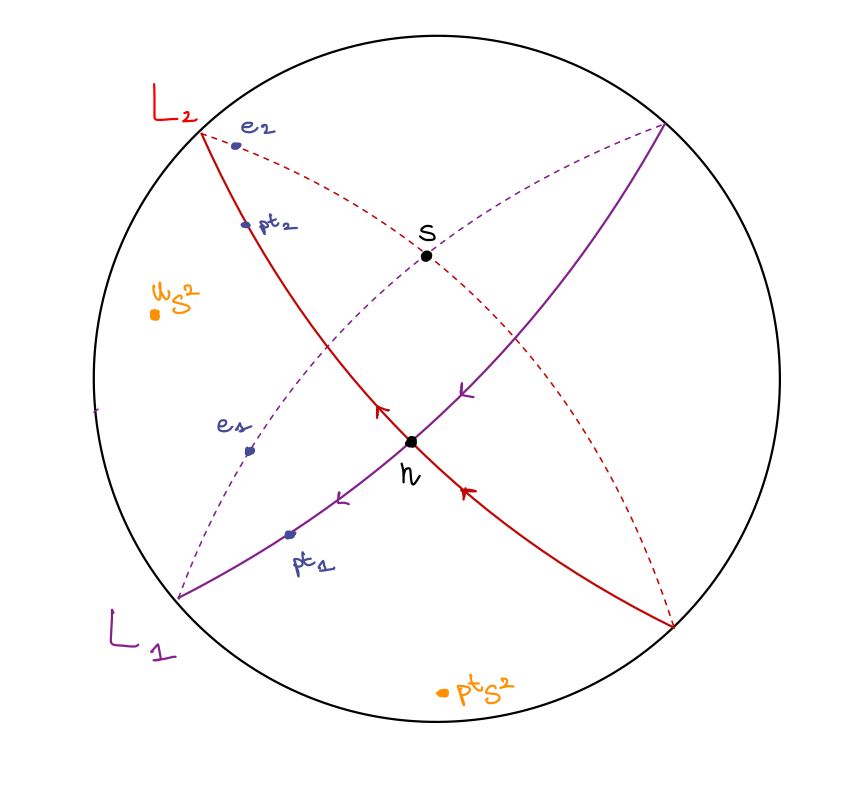
\includegraphics[scale=0.3]{S2approx.png}
	\centering
	\caption{The geometric situation described in Proposition \ref{OCS2} in the case $N=2$.} \label{fig:S2approx}
\end{figure}
\begin{rem}
\begin{proof}
	%Recall that the $p$-Floer complex of any two transversally intersecting Lagrangians is generated by their intersection points, all set at action $\nu(p)$ by definition of our class of Floer data (see Definition \ref{FD}).
	We will number our equators so that looking from the north pole, they are ordered clockwise starting from $L_1$. We drop $p$ from the notation and write $C_i:=CF(L_{i},L_{i+1})$ and $C_i':= CF(L_{i+1},L_i)$ for any $i=1,\ldots, N$\footnote{With the convention $L_{N+1}=L_1$.}. For any $i$, we denote by $n_i, s_i \in C_i$  and $n_i',s_i'\in C_i'$ the north and south poles respectively. To simplify the computations in the remainings of the proof, we impose the following additional restrictions on the functions $f^{L_i}_p$ in the $p$-Floer datum of each equator $L_i$: we require that flowing from the north pole to the south pole, one encounters first $\text{pt}_i$ and then $e_i$, before getting to the south pole. We also require that the critical points $u_{S^2}$ and $\text{pt}_{S^2}$ of the Morse function $f^{S^2}_p$ in the $p$-Floer datum of the ambient manifold $f_p^{S^2}\colon S^2\to \mathbb{R}$ both lie in the area between $L_1$ and $L_2$, but not on $L_1$ or $L_2$.
	
	We claim that $$\vec{\gamma}:=\sum_{i=1}^N n_i\otimes s_i'\in \bigoplus_{i=1}^N C_i\otimes C_i'\subset CC_*(\mathcal{E}(N))$$ is a Hochschild cycle, and moreover $$OC_p^{\mathcal{E}(N)}\left(\sum_{i=1}^N n_i\otimes s_i'\right)=T^{\frac{1}{2N}}u_M.$$ This would prove the statement as $$\mathbb{A}_{CC}\left(\sum_{i=1}^N n_i\otimes s_i'\right) = \mathbb{A}_{CC}(n_i\otimes s_i') = \mathbb{A}(n_i)+\mathbb{A}(s_i')\leq 2\nu(p)$$ by definition of the filtration on the Hochschild complex.
	
	We first prove that $\vec{\gamma}$ is a Hochschild cycle. Let $i\in\{1,\ldots, N\}$. We compute $$\mu_2(n_i,s_i') = T^{\frac{1}{2N}}e_i \text{  and  } \mu_2(s_i',n_i) = T^{\frac{1}{2N}}e_{i+1}$$ by just counting slices of the sphere as in Figure \ref{fig:S2approx}. By definition of the Hochschild differential we then have $$d_{CC}(n_i\otimes s_i')=T^{\frac{1}{2N}}(e_i+e_{i+1}),$$ hence $$d_{CC}(\vec{\gamma}) = T^{\frac{1}{2N}}\sum_{i=1}^N \left(e_i+e_{i+1}\right) = 0$$ as we work with $\mathbb{Z}_2$ coefficients. This shows that $\vec{\gamma}$ is an Hochschild cycle.
	
	The computation of $OC_p^{\mathcal{B}}(\vec{\gamma})$ is easy in this setting. Because of the choice of $f^{S^2}_p$ we have $$OC_p^\mathcal{B}(\vec{\gamma}) = OC_p^\mathcal{B}(n_1\otimes s_1') = T^{\frac{1}{2N}}u_{S^2}$$ by degree reasons.
\end{proof}

	Another way to prove the above proposition is to show that the element $\vec{\gamma}$ is homologous, in $CC(\mathcal{E}(N))$, to $T^{-\frac{N-1}{2N}}\text{pt}_{L_i}\otimes \text{pt}_{L_i}\in CF(L_i,L_i)\otimes CF(L_i,L_i)$ for any $i$.
\end{rem}


%=======================================
%=======================================
%=======================================


\subsubsection{Approximability of non-contractible circles on the $2$-torus}
Consider the standard symplectic $2$-torus $\mathbb{T}^2=\mathbb{R}^2/\mathbb{Z}^2$ with unit volume. We are interested in the class of non-contractible Lagrangians $\lagwex(\mathbb{T}^2)$. We will use coordinates $(x,y)$ on $\mathbb{T}^2$ and denote by $(n,m)$ the lattice coordinates on $\mathbb{Z}^2$. We recall that, for us, the weakly exact case is a particular instance of the monotone setting. %The main result of this section is the following.
%\begin{thm}\label{retractapproxt2}	The set of non-contractible Lagrangians $\lagwex(\mathbb{T}^2)$ of the $2$-torus is Fukaya retract-approximable.\end{thm}

We introduce the following notation: $$L_y:=\{x=0\}\subset \mathbb{T}^2\text{    and    }L^\theta_x:=\{y=\theta\}\subset \mathbb{T}^2 \text{  for any $\theta\in S^1$} $$ and denote the unique intersection point between $L_y$ and $L_x^\theta$ by $a^\theta\in L^\theta_x\pitchfork L_y.$ We denote $L_x:=L_x^0$ and $a:=a^0$. In this section, we will work with the family $$\mathcal{N}:=\{L_y\}\cup\{L_x^\theta\bigm| \theta\in S^1\}\subset \lagwex(\mathbb{T}^2).$$ %of non-contractible circles on $\mathbb{T}^2$ containing $L_y$ and $L_x^\theta$ for all $\theta \in S^1$. 
We will write $a^\theta$ seen as the generator of Floer complexes as $$a^\theta_{xy}\in CF(L^\theta_x,L_y) \text{   and   } a^\theta_{yx}\in CF(L_y,L^\theta_x)$$ for any choice of perturbation datum $p\in \mathcal{P}$, which we omit from the notation. In this section, we will only consider (without loss of generality) perturbation data $p\in \mathcal{P}$ satisfying the following:
\begin{enumerate}
	\item Consider the Morse function $f^{\mathbb{T}^2}_p\colon \mathbb{T}^2\to \mathbb R$ in the $p$-Floer datum for $\mathbb{T}^2$. We assume that $f^{\mathbb{T}^2}_p$ has exactly four critical points: a unique maximum $u_{\mathbb{T}^2}\in \mathbb{T}^2$, two saddle points $s_1,s_2\in \mathbb{T}^2$ and a unique minimum $\text{pt}_{\mathbb{T}^2}\in \mathbb{T}^2$. We further assume that all these critical points do not lie on the Lagrangian $L_y$ introduced above.
	\item Let $L\in \lagwex(\mathbb{T}^2)$ and consider the Morse function $f^L_p\colon L\to \mathbb{R}$ in the $p$-Floer datum of $L$. We assume that $f^L_p$ has a unique maximum $e_L\in L$ and a unique minimum $\text{pt}_L\in L$. We will always assume that both $e_L$ and $\text{pt}_L$ do not lie on the Lagrangian $L_y$ introduced above. In the special cases where $L$ is one of the Lagrangians $L_y$ or $L_x^\theta$ in $\mathcal{N}$, we denote the critical points as $e_y$, $pt_y$ or $e_x^\theta$, $pt_y^\theta$.
\end{enumerate}
\begin{rem}
	The role of $x$ and $y$ are intercheangeable. Moreover, we could work with the countable subfamily $\mathcal{N}_c$ containing $L_y$ and $L_x^\theta$ for all $\theta \in \mathbb{Q}/\mathbb{Z}$.
\end{rem}

As for the case of the $2$-sphere in the subsection above, we first prove a warm up low-accuracy retract-approximation result, before moving to a more general case. In the following proposition we will work with the Lagrangian $L_x$, but the same results hold for all $L_x^\theta$.
\begin{prop}
	Let $p\in \mathcal{P}$. Then $\lagwex(\mathbb{T}^2)$ is retract approximable in $\mathcal{A}_p$ by $\mathcal{B}_{xy}:=\{L_x,L_y\}$ with accuracy $\frac{1}{2}+3\nu(p)$.
\end{prop}
\begin{proof}
	Consider the Hochschild chain $\vec{a}=a_{xy}\otimes a_{yx}\otimes a_{xy}\otimes a_{yx}\in CC_*(\mathcal{B}_{xy})$. We show it is a cycle. For this, we compute all possible cyclic partial contractions.
	\begin{enumerate}
		\item First, both $\mu_2(a_{xy},a_{yx})\in CF(L_x,L_x)$ and $\mu_2(a_{yx},a_{xy})\in CF(L_y,L_y)$ vanish, as the only allowed contributions are Morse trajectories to $\text{pt}_x$ and $\text{pt}_y$ respectively, which come in pairs.
		\item The terms $\mu_3(a_{xy},a_{yx},a_{xy})\in CF(L_x,L_y)$ and $\mu_3(a_{yx},a_{xy},a_{yx})$ vanish as well. For instance, $$\mu_3(a_{xy},a_{yx},a_{xy}) = 2\sum_{n,m>0}T^{nm}a_{xy}$$ as we can see the "two opposite" $a_{xy}$ in the fundamental square of $\mathbb{T}^2$ as exits in two different ways (for each lattice-polygon $(n,m)$).
		\item The terms $\mu_4(a_{xy},a_{yx},a_{xy},a_{yx})\in CF(L_x,L_x)$ and $\mu_4(a_{yx},a_{xy},a_{yx},a_{x,y})\in CF(L_y,L_y)$ both vanish. For instance $$\mu_4(a_{xy},a_{yx},a_{xy},a_{yx})=2\sum_{n,m>0}nT^{nm}e_x$$ since in a lattice polygon of width $n$ we can have $e_x$ as an exit in $2n$ different ways.
	\end{enumerate}
	It follows that $\vec{a}\in CC_*(B_{xy})$ is a cycle. We compute $$OC^{\mathcal{B}_{xy}}(\vec{a}) = \sum_{n,m>0}nmT^{nm}u_{\mathbb{T}^2}$$ since in every $(n,m)$ lattice polygon we can see $u$ as an exit in $nm$ different position (one for every fundamental square embedded in the polygon). Since we are working over $\mathbb{Z}_2$ it follows that $$OC^{\mathcal{B}_{xy}}(\vec{a}) = \sum_{n>0}n^2T^{n^2}u_{\mathbb{T}^2} =  \sum_{n\geq0}T^{(2n+1)^2}u_{\mathbb{T}^2}.$$ Note that the smallest Novikov exponent in this expression is $1$. Since intersection points lie at filtration level $\leq \nu(p)$ by definition, the claim follows.
\end{proof}
\begin{rem}
	More formally, given the Novikov element $$f(T)= \sum_{n\geq0}T^{(2n+1)^2}$$ we have $$f^{-1}(T) = T^{-1}\sum_{n\geq 0}g_nT^n$$ where $g_0=1$ and $$g_n = \sum_{e\in E\setminus\{0\}, \ e\leq n}g_{n-e}$$ where $E= \{(2n+1)^2-1\ : \ n\geq 0\}$. Indeed, writing $\frac{f(T)}{T}= \sum_{n\geq 0}f_nT^n$ where $f_n =1 $ if and only if $n\in E$, we have that $f_0\cdot g_0=1$ while the coefficient of $T^n$ for $n\geq 1$ in $f\cdot f^{-1}$ is 
	\begin{align*}
		\sum_{j=1}^nf_jg_{n-j} = \sum_{j\in E, \ j\leq n}g_{n-j} = g_n+  \sum_{j\in E\setminus\{0\}, \ j\leq n}g_{n-j}=0
	\end{align*}
	It follows directly from our definition of the action filtration on $\Lambda$, that $f^{-1}\in \Lambda$ lies at filtration level $\leq 1$.\\
	Using the formalism of theta-functions we can write $$\sum_{n\geq 0}T^{(2n+1)^2}= \sum_{n\in \mathbb Z}T^{(4n+1)^2}=\theta_{\frac{1}{4},0}(16,0).$$ But also notice that $$\sum_{n\geq 0}n^2T^{n^2}=T\theta'_{0,0}(1,0)$$
\end{rem}
\begin{prop}\label{prop235}
	Let $p\in \mathcal{P}$ and and $N\geq 1$. Consider the family $\mathcal{N}(N)= \{L_y,L_1,\ldots, L_N\}\subset \mathcal{N}$, where $$L_j=L_x^{\frac{j-1}{N}}$$ for $j=1,\ldots, N$. $\lagwex(\mathbb{T}^2)$ is retract approximable in $\mathcal{A}_p$ by $\mathcal{N}(N)$ with accuracy $\frac{1}{2N}+ 3\nu(p)$.%Then $\mathcal{N}(N)$ retract-approximates $\mathcal{L}^{we}(\mathbb{T}^2)$ with accuracy $\frac{1}{N}+ 4\nu(p)$ in $\mathcal{C}\mathcal{F}uk(\mathbb{T}^2,p)$.
\end{prop}
%\begin{figure}
%	\includegraphics[scale=0.3]{T2.png}
%	\centering
%
%\end{figure}

%\begin{figure}[ht]
%	\centering
%\begin{tikzpicture}[x=1cm,y=1cm, line cap=round, line join=round]
%	
%	% --- Colors
%	\definecolor{myPurple}{RGB}{102,0,153}
%	\definecolor{myOrange}{RGB}{230,140,20}
%	\definecolor{myGreen}{RGB}{90,170,70}
%	
%	% --- Geometry (SQUARE)
%	\def\xL{0}
%	\def\xR{7}    % square: width = height = 7
%	
%	\def\yTop{7.0}
%	\def\yA{5.6}
%	\def\yB{4.9}
%	\def\yC{3.2}
%	\def\yD{2.4}
%	\def\yE{1.1}
%	\def\yBot{0.0}
%	
%	% --- Orange vertical sides
%	\draw[myOrange, line width=3pt] (\xL,\yBot) -- (\xL,\yTop);
%	\draw[myOrange, line width=3pt] (\xR,\yBot) -- (\xR,\yTop);
%	
%	% --- Helper: horizontal line + endpoints
%	\newcommand{\hlinewithdots}[1]{%
%		\draw[myPurple, line width=3pt] (\xL,#1) -- (\xR,#1);
%		\fill[black] (\xL,#1) circle (1.6pt);
%		\fill[black] (\xR,#1) circle (1.6pt);
%	}
%	
%	% --- Horizontal lines
%	\hlinewithdots{\yTop}
%	\hlinewithdots{\yA}
%	\hlinewithdots{\yB}
%	\hlinewithdots{\yC}
%	\hlinewithdots{\yD}
%	\hlinewithdots{\yE}
%	\hlinewithdots{\yBot}
%	
%	% --- Interior points
%	\fill[myPurple] (2.0,\yTop) circle (1.4pt);
%	\fill[myPurple] (4.8,\yTop) circle (1.4pt);
%	
%	\fill[myPurple] (2.1,\yBot) circle (1.4pt);
%	\fill[myPurple] (4.9,\yBot) circle (1.4pt);
%	
%	% --- Vertical dots
%	\foreach \yy in {6.4,6.2,6.0} { \fill[myPurple] (3.5,\yy) circle (1.1pt); }
%	\foreach \yy in {4.1,3.9,3.7} { \fill[myPurple] (3.5,\yy) circle (1.1pt); }
%	\foreach \yy in {2.0,1.8,1.6} { \fill[myPurple] (3.5,\yy) circle (1.1pt); }
%	
%	% --- Left labels
%	\node[myOrange, anchor=south west, scale=1.2] at (-0.3,\yTop) {$L_y$};
%	
%	\fill[myOrange] (\xL, {(\yA+\yB)/2}) circle (2.5pt);
%	\node[myOrange, anchor=east, scale=1.1] at (-0.2, {(\yA+\yB)/2}) {$e_y$};
%	
%	\node[black, anchor=east, scale=1.2] at (-0.25,\yBot) {$a^1$};
%	\node[black, anchor=east, scale=1.2] at (-0.25,\yE) {$a^2$};
%	\node[black, anchor=east, scale=1.2] at (-0.25,\yD) {$a^i$};
%	\node[black, anchor=east, scale=1.3] at (-0.35,{(\yE+\yD)/2}) {$\vdots$};
%	\node[black, anchor=east, scale=1.3] at (-0.35,{(\yB+\yC)/2}) {$\vdots$};
%	
%	% --- Right labels
%	\node[myPurple, anchor=west, scale=1.2] at (\xR+0.25,\yTop) {$L_1$};
%	\node[myPurple, anchor=west, scale=1.2] at (\xR+0.25,\yA) {$L_{\ell+1}$};
%	\node[myPurple, anchor=west, scale=1.2] at (\xR+0.25,\yB) {$L_{\ell}$};
%	\node[myPurple, anchor=west, scale=1.2] at (\xR+0.25,\yC) {$L_{i+1}$};
%	\node[myPurple, anchor=west, scale=1.2] at (\xR+0.25,\yD) {$L_i$};
%	\node[myPurple, anchor=west, scale=1.2] at (\xR+0.25,\yE) {$L_2$};
%	\node[myPurple, anchor=west, scale=1.2] at (\xR+0.25,\yBot) {$L_1$};
%	
%	% --- Green point
%	\fill[myGreen] (4.1,2.85) circle (1.6pt);
%	\node[myGreen, anchor=west, scale=1.2] at (4.3,2.85) {$u_{\mathbb{T}^2}$};
%	
%	% --- Bottom labels
%	\node[myPurple, anchor=north, scale=1.2] at (2.1,-0.25) {$\text{pt}_1$};
%	\node[myPurple, anchor=north, scale=1.2] at (4.9,-0.25) {$e_1$};
%	
%	
%	% --- Purple dots on top & bottom lines (interior)
%	\fill[myPurple] (2,\yTop) circle (2.1pt);
%	\fill[myPurple] (4.85,\yTop) circle (2.1pt);
%	
%	\fill[myPurple] (2,\yBot) circle (2.1pt);
%	\fill[myPurple] (4.85,\yBot) circle (2.1pt);
%	
%\end{tikzpicture}
%	\caption{The fundamental domain of $\mathbb{T}^2$ with the approximating family of Lagrangians $\mathcal{N}(N)$ discussed in Proposition \ref{prop235}.} \label{fig:T2approx}
%\end{figure}
\begin{figure}
	\centering
	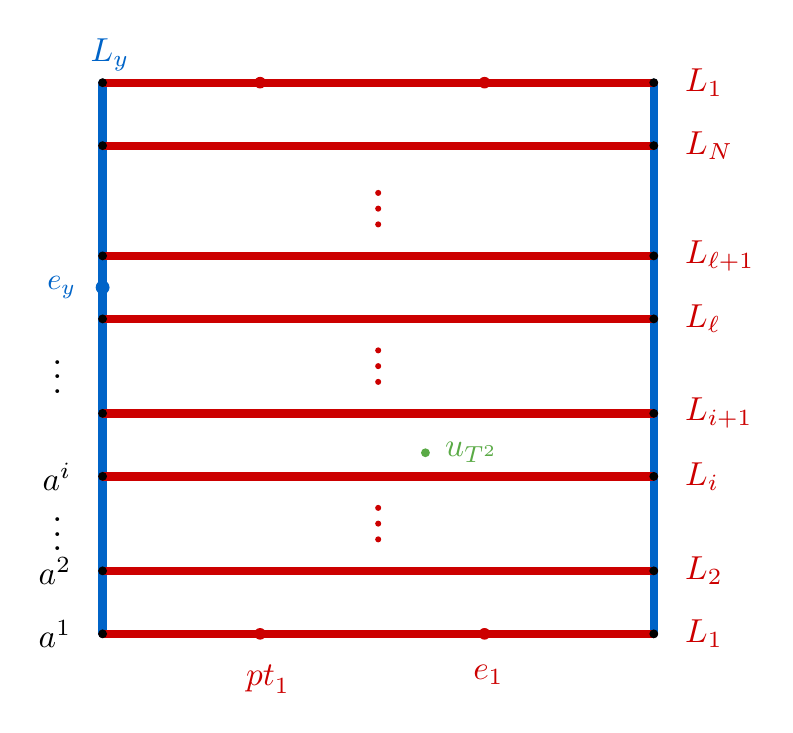
\begin{tikzpicture}[x=1cm,y=1cm, line cap=round, line join=round]
		
		% --- Colors
		\definecolor{myPurple}{RGB}{204,0,0}
		\definecolor{myOrange}{RGB}{0,100,200}
		\definecolor{myGreen}{RGB}{90,170,70}
		
		% --- Geometry (SQUARE)
		\def\xL{0}
		\def\xR{7}    % square: width = height = 7
		
		\def\yTop{7.0}
		\def\yAA{6.2}
		\def\yA{4.8}
		\def\yB{4}
		\def\yC{2.8}
		\def\yD{2}
		\def\yE{0.8}
		\def\yBot{0.0}
		
		% --- Orange vertical sides
		\draw[myOrange, line width=3pt] (\xL,\yBot) -- (\xL,\yTop);
		\draw[myOrange, line width=3pt] (\xR,\yBot) -- (\xR,\yTop);
		
		% --- Helper: horizontal line + endpoints
		\newcommand{\hlinewithdots}[1]{%
			\draw[myPurple, line width=3pt] (\xL,#1) -- (\xR,#1);
			\fill[black] (\xL,#1) circle (1.6pt);
			\fill[black] (\xR,#1) circle (1.6pt);
		}
		
		% --- Horizontal lines
		\hlinewithdots{\yTop}
		\hlinewithdots{\yAA}
		\hlinewithdots{\yA}
		\hlinewithdots{\yB}
		\hlinewithdots{\yC}
		\hlinewithdots{\yD}
		\hlinewithdots{\yE}
		\hlinewithdots{\yBot}
		
		% --- Interior points
		\fill[myPurple] (2.0,\yTop) circle (1.4pt);
		\fill[myPurple] (4.8,\yTop) circle (1.4pt);
		
		\fill[myPurple] (2.1,\yBot) circle (1.4pt);
		\fill[myPurple] (4.9,\yBot) circle (1.4pt);
		
		% --- Vertical dots
		\foreach \yy in {5.6,5.4,5.2} { \fill[myPurple] (3.5,\yy) circle (1.1pt); }
		\foreach \yy in {3.6,3.4,3.2} { \fill[myPurple] (3.5,\yy) circle (1.1pt); }
		\foreach \yy in {1.6,1.4,1.2} { \fill[myPurple] (3.5,\yy) circle (1.1pt); }
		
		% --- Left labels
		\node[myOrange, anchor=south west, scale=1.2] at (-0.3,\yTop) {$L_y$};
		
		\fill[myOrange] (\xL, {(\yA+\yB)/2}) circle (2.5pt);
		\node[myOrange, anchor=east, scale=1.1] at (-0.2, {(\yA+\yB)/2}) {$e_y$};
		
		\node[black, anchor=east, scale=1.2] at (-0.25,\yBot) {$a^1$};
		\node[black, anchor=east, scale=1.2] at (-0.25,\yE) {$a^2$};
		\node[black, anchor=east, scale=1.2] at (-0.25,\yD) {$a^i$};
		\node[black, anchor=east, scale=1.3] at (-0.35,{(\yE+\yD)/2}) {$\vdots$};
		\node[black, anchor=east, scale=1.3] at (-0.35,{(\yB+\yC)/2}) {$\vdots$};
		
		% --- Right labels
		\node[myPurple, anchor=west, scale=1.2] at (\xR+0.25,\yTop) {$L_1$};
		\node[myPurple, anchor=west, scale=1.2] at (\xR+0.25,\yAA) {$L_{N}$};
		\node[myPurple, anchor=west, scale=1.2] at (\xR+0.25,\yA) {$L_{\ell+1}$};
		\node[myPurple, anchor=west, scale=1.2] at (\xR+0.25,\yB) {$L_{\ell}$};
		\node[myPurple, anchor=west, scale=1.2] at (\xR+0.25,\yC) {$L_{i+1}$};
		\node[myPurple, anchor=west, scale=1.2] at (\xR+0.25,\yD) {$L_i$};
		\node[myPurple, anchor=west, scale=1.2] at (\xR+0.25,\yE) {$L_2$};
		\node[myPurple, anchor=west, scale=1.2] at (\xR+0.25,\yBot) {$L_1$};
		
		% --- Green point
		\fill[myGreen] (4.1,2.3) circle (1.6pt);
		\node[myGreen, anchor=west, scale=1.2] at (4.2,2.3) {$u_{\mathbb{T}^2}$};
		
		% --- Bottom labels
		\node[myPurple, anchor=north, scale=1.2] at (2.1,-0.25) {$\text{pt}_1$};
		\node[myPurple, anchor=north, scale=1.2] at (4.9,-0.25) {$e_1$};
		
		
		% --- Purple dots on top & bottom lines (interior)
		\fill[myPurple] (2,\yTop) circle (2.1pt);
		\fill[myPurple] (4.85,\yTop) circle (2.1pt);
		
		\fill[myPurple] (2,\yBot) circle (2.1pt);
		\fill[myPurple] (4.85,\yBot) circle (2.1pt);
		
	\end{tikzpicture}
	\caption{The fundamental domain of $\mathbb{T}^2$ with the approximating family of Lagrangians $\mathcal{N}(N)$ discussed in Proposition \ref{prop235}.} \label{fig:T2approx}
\end{figure}
%3D PICTURE
%\begin{figure}
%	\centering
%	\tdplotsetmaincoords{70}{115}
%	
%	\begin{tikzpicture}[tdplot_main_coords, line cap=round, line join=round, scale=1.25]
%		
%		% --- Colors (same as your figure)
%		\definecolor{myPurple}{RGB}{102,0,153}
%		\definecolor{myOrange}{RGB}{230,140,20}
%		
%		% --- Radii
%		\def\R{2.3}   % major radius
%		\def\r{0.85}  % minor radius
%		
%		% --- Styles
%		\tikzset{
%			purpleloop/.style={myPurple, line width=1.4pt},
%			orangeloop/.style={myOrange, line width=2.2pt},
%			faint/.style={black, opacity=0.18, line width=0.4pt},
%		}
%		
%		% (Optional) faint torus grid for 3D readability
%		\foreach \vv in {0,45,90,135} {
%			\draw[faint]
%			plot[variable=\uu, domain=0:360, samples=140]
%			({(\R+\r*cos(\vv))*cos(\uu)},
%			{(\R+\r*cos(\vv))*sin(\uu)},
%			{\r*sin(\vv)});
%		}
%		\foreach \uu in {0,60,120,180,240,300} {
%			\draw[faint]
%			plot[variable=\vv, domain=0:360, samples=140]
%			({(\R+\r*cos(\vv))*cos(\uu)},
%			{(\R+\r*cos(\vv))*sin(\uu)},
%			{\r*sin(\vv)});
%		}
%		
%		% --- Many PURPLE circles: fix v, vary u  (like horizontal lines in the square)
%		% --- Many PURPLE circles: fix v, vary u  (FULL 0..360 coverage)
%		\foreach \vv in {0,20,40,60,80,100,120,140,160,180,200,220,240,260,280,300,320,340} {
%			\draw[purpleloop]
%			plot[variable=\uu, domain=0:360, samples=180]
%			({(\R+\r*cos(\vv))*cos(\uu)},
%			{(\R+\r*cos(\vv))*sin(\uu)},
%			{\r*sin(\vv)});
%		}
%		
%		
%		% --- One ORANGE circle: fix u, vary v  (one vertical direction cycle)
%		\def\uOrange{35} % pick where it sits (degrees)
%		\draw[orangeloop]
%		plot[variable=\vv, domain=0:360, samples=220]
%		({(\R+\r*cos(\vv))*cos(\uOrange)},
%		{(\R+\r*cos(\vv))*sin(\uOrange)},
%		{\r*sin(\vv)});
%		
%	\end{tikzpicture}
%	\caption{AA}
%\end{figure}

\begin{proof}
	We assume that the critical point $u_{\mathbb{T}^2}$ doesn't lie on any Lagrangian in $\mathcal{N}(N)$. We denote by $e_j\in CF(L_j,L_j)$ and $\text{pt}_j\in CF(L_j,L_j)$ the maximum and the minimum of the Morse function $f_p^{L_j}$ for any $j=1,\ldots, N$. Moreover, for any $j$, we denote by $a^j_{xy}\in CF(L_j,L_y)$ and $a^j_{yx}\in CF(L_y,L_j)$ the intersection point $a$ seen as a generator of the Floer complexes. We denote by $i\in \{1,\ldots, N\}$ the unique index such that $u_{\mathbb{T}^2}$ lies in the area between $L_i$ and $L_{i+1}$. Similarly, we denote by $l$ the unique index such that $e_y\in CF(L_y,L_y)$ lies in the $L_y$-segment between $L_l$ and $L_{l+1}$. Figure \ref{fig:T2approx} provides a schematic depiction of the geometric setup.
	
	For any $j=1,\ldots, N$, consider the Hochschild chain\footnote{Here $N+1=1$.} $$\gamma^j:=a^j_{xy}\otimes a^{j+1}_{yx}\otimes a^{j+1}_{xy}\otimes a^{j}_{yx}\in CC_*(\mathcal{N}(N)).$$ Given a real number $A\in \mathbb{R}$, let\footnote{Here $h$ stands for \textit{horizontal} and $v$ for \textit{vertical.}} $$q^h_{A}(T):= \sum_{n,m>0}n(T^{n(m-1+A)}+ T^{n(m-A)}) \text{   and   } \tilde{q}^h_{\frac{1}{N}}(T):`= \sum_{n,m>0}T^{n(m-1+A)}+ T^{n(m-A)}$$ as well as 
	$$q^v_A(T):= \sum_{n,m>0}m(T^{n(m-A)}+ T^{n(m+A)}) \text{   and   } \tilde{q}^v_A(T):= \sum_{n,m>0}T^{n(m-A)}+ T^{n(m+A)} $$ be elements of the Novikov field $\Lambda$. We compute the Hochschild differential of $\gamma^j$ by computing all possible contractions. 
	\begin{enumerate}
		\item We have $$\mu_4(a^{j}_{xy},a^{j+1}_{yx}, a^{j+1}_{xy}, a^{j}_{yx}) = q^h_{\frac{1}{N}}(T)e_j\text{   and   } \mu_4(a^{j+1}_{xy},a^{j}_{yx},a^{j}_{xy},a^{j+1}_{yx})= q^h_{\frac{1}{N}}(T)e_{j+1},$$ while $$\mu_4(a^{j}_{yx},a^{j}_{xy},a^{j+1}_{yx}, a^{j+1}_{xy}) = \mu_4(a^{j+1}_{yx},a^{j+1}_{xy},a^{j}_{yx},a^{j}_{xy})= \begin{cases}
			q^v_{\frac{1}{N}}(T) e_y, \text{  if }j\neq l\\
			q^v_{1-\frac{1}{N}}(T)e_y, \text{  if }j=l.
		\end{cases} $$ %$$\mu_4(a^{j}_{yx},a^{j}_{xy},a^{j+1}_{yx}, a^{j+1}_{xy}) = \mu_4(a^{j+1}_{yx},a^{j+1}_{xy},a^{j}_{yx},a^{j}_{xy})= \begin{cases}                \sum_{n,m>0}m(T^{n(m-\frac{1}{N})}+ T^{n(m+\frac{1}{N})})e_y, \text{  if }j\neq l\\                \sum_{n,m>0}m(T^{n(m+\frac{1}{N}-1)}+ T^{n(m+1-\frac{1}{N})})e_y, \text{  if }j=l            \end{cases} $$ 
		\item We have $$\mu_3(a^{j}_{xy},a^{j+1}_{yx}, a^{j+1}_{xy}) = \tilde{q}^h_{\frac{1}{N}}(T)a^j_{xy} \text{   and   }\mu_3(a^{j+1}_{yx},a^{j+1}_{xy},a^{j}_{yx}) = \tilde{q}^h_{\frac{1}{N}}(T)a^{j}_{yx}$$
		while $$\mu_3(a^{j}_{yx},a^{j}_{xy},a^{j+1}_{yx}) = \tilde{q}^h_{\frac{1}{N}}(T)a^{j+1}_{yx} \text{   and   }\mu_3(a^{j+1}_{xy},a^j_{yx},a^{j}_{xy}) = \tilde{q}^h_{\frac{1}{N}}(T)a^{j+1}_{xy}$$
		
	\end{enumerate}
	We now compute the relevant $\mu_3$'s.
	It follows that \begin{align*}
		d_{CC}(\gamma^j) & = q^h_{\frac{1}{N}}(T)(e_j+e_{j+1}) + 2q^v_{c_j}(T)e_y + \tilde{q}^h_{\frac{1}{N}}(T)(2a^j_{xy}\otimes a^j_{yx} + a^{j+1}_{xy}\otimes a^{j+1}_{yx} + a^{j+1}_{yx}\otimes a^{j+1}_{xy}) \\ & = q^h_{\frac{1}{N}}(T)(e_j+e_{j+1}) + \tilde{q}^h_{\frac{1}{N}}(T)(a^{j+1}_{xy}\otimes a^{j+1}_{yx} + a^{j+1}_{yx}\otimes a^{j+1}_{xy})
	\end{align*}
	where $c_j = \frac{1}{N}$ if $j\neq l$ and $c_j=1-\frac{1}{N}$ otherwise.
	Hence $$d_{CC}\left(\sum_{j=1}^N \gamma^j\right) =  \tilde{q}^h_{\frac{1}{N}}(T)\sum_{j=1}^N(a^{j}_{xy}\otimes a^{j}_{yx} + a^{j}_{yx}\otimes a^{j}_{xy}) $$ as by summing over $j$ the summands of the form $e_j$ cancel out in pairs. In particular, $\sum_{j=1}^N\gamma^j$ is not a cycle. However, we claim that $$\vec{\gamma} = \sum_{j=1}^N\gamma^j + \tilde{q}^h_{\frac{1}{N}}(T)\ e_j\otimes a^j_{xy}\otimes a^j_{yx}\in CC_*(\mathcal{N}(N))$$ is a cycle. Indeed: $$d_{CC}(e_j\otimes a^j_{xy}\otimes a^j_{yx}) = \mu_2(e_j,a^j_{xy})\otimes a^j_{yx} + \mu_2(a^j_{yx},e_j)\otimes a^j_{xy} =a^{j}_{xy}\otimes a^{j}_{yx} + a^{j}_{yx}\otimes a^{j}_{xy},$$ since $e_j$ is a strict unit and the product of the point with itself vanishes.\\
	
	We now compute $OC^{\mathcal{N}(N)}(\vec{\gamma})\in CQ(\mathbb{T}^2)$. Recall that $i\in \{1,\ldots, N\}$ is defined as the only index such that the critical point $u=u_{\mathbb{T}^2}$ of the Morse function $f^{\mathbb{T}^2}_p$ used to define $QH_*(M)$ lies in the area between $L_i$ and $L_{i+1}$. Let $j\in \{1,\ldots, N\}$, then \begin{align*}
		OC(\gamma^j) &= \begin{cases}
			\sum_{n,m>0}nm(T^{n(m-\frac{1}{N})}+T^{n(m+\frac{1}{N})})u,  \text{ if }j\neq i\\
			\sum_{n,m>0}nm(T^{n(m-1+\frac{1}{N})}+T^{n(m+1-\frac{1}{N})})u,  \text{ if }j=i
		\end{cases}
	\end{align*}
	On the other hand, for all $j\in \{1,\ldots, N\}$ it is easy to see that we have $$OC(e_j\otimes a^j_{xy}\otimes a^j_{yx}) =0.$$ If $N$ is odd, then we have $$OC(\vec{\gamma}) = OC(\gamma^i) = \sum_{k\geq 0}\sum_{\substack{d=\pm 1 \ (2N)\\ d|2k+1}}T^{\frac{2k+1}{N}}$$ while if $N$ is even we have, for some $j\neq i$: $$OC(\vec{\gamma}) = OC(\gamma^i)+OC(\gamma^j) = \sum_{k\geq 0}\sum_{\substack{d=\pm 1, \pm1+N \ (2N)\\ d|2k+1}}T^{\frac{2k+1}{N}}$$
	%If $N$ is odd, then $$OC(\vec{\gamma}) = OC(\gamma^i)$$ since all other contributions cancel out over $\Z_2$. If $N$ is even, we have $$OC(\vec{\gamma}) = $$
	In all cases the lowest order term is $T^{\frac{1}{N}}u_{\mathbb{T}^2}$. The claim follows.
	
\end{proof}

%\begin{proof}[Proof of Theorem \ref{retractapproxt2}]	Let $\Delta>0$ and consider the family $\mathcal{N}=\{L_y\}\cup \{L_x^\theta \ : \ \theta \in S^1\}$ introduced above. We choose a subset $\mathcal{N}(N)$ of cardinality $N+1$ as in Proposition \ref{prop235}. Then for any filtered perturbation datum $p$ as in the proof of proposition \ref{prop235} of size $\nu(p)<\frac{1}{4}(\delta-\frac{1}{N})$, the family $\mathcal{L}^{we}(\mathbb{T}^2)$ of non-contractible Lagrangians on $\mathbb{T}^2$ is retract approximated by $\mathcal{N}(N)$ with accuracy $\delta$ in the TPC $\mathcal{C}\mathcal{F}uk(\mathbb{T}^2,p)$.\end{proof}

In Proposition \ref{prop235} we worked with only one Lagrangian in the $y$ direction. We can generalize the result to families containing $N+M$ circles, $N$ in the $x$ direction and $M$ in the $y$ direction, to get retract-approximation of order $\frac{1}{NM}$. Below we prove this for $N=M$.

\begin{prop}
	Let $p\in \mathcal{P}$ and $N\geq 1$. Consider the family $$\mathcal{N}(N)= \{L^1_y,\ldots, L_y^N,L_x^1,\ldots, L_x^N\}\subset \mathcal{N},$$ where $$L_y^j:= L_y^{\frac{j-1}{N}}\text{    and    }L_x^j=L_x^{\frac{j-1}{N}}$$ for $j=1,\ldots, N$. Then $\mathcal{N}(N)$ retract-approximates $\mathcal{L}^{we}(\mathbb{T}^2)$ with accuracy $\frac{1}{2N^2}+ 3\nu(p)$ in $\mathcal{A}_p$.
\end{prop}
\begin{proof}
	Essentially, the proof is the same as Proposition \ref{prop235}. We denote by $a^{j,k}$ the unique intersection point in $L_x^j\cap L_y^k$ and write it as $a^{j,k}_{xy}$ when seen as a generator of $CF(L_x^j,L_y^k)$ and as $a^{j,k}_{y,x}$ when seen as a generator of $CF(L_y^k,L_x^j)$. Let $i_x$ and $i_y$ the only indices such that the critical point $u=u_{\mathbb{T}^2}$ of the Morse function defining $QH(\mathbb{T}^2)$ lies in the square bounded by the Lagrangians $L_x^{i_x}$, $L_x^{i_x+1}$, $L_y^{i_y}$ and $L_y^{i_y+1}$. The key fact is that 
	\begin{align*}
		OC(a^{i_x,i_y}_{xy}\otimes a^{i_y,i_x+1}_{yx}\otimes a^{i_x+1,i_y+1}_{xy}\otimes a^{i_y+1,i_x}_{yx})&=\sum_{n,m>0}nm(T^{(n-1+\frac{1}{N})(m-1+\frac{1}{N}}+T^{(n+1-\frac{1}{N})(m+1-\frac{1}{N}})u \\& =\sum_{n>0}n^2(T^{(n-1+\frac{1}{N})^2}+T^{(n+1-\frac{1}{N})^2})u\\ & = \sum_{n\geq 0}T^{(2n+\frac{1}{N})^2}+T^{(2n+2-\frac{1}{N})^2}u\\ & = \sum_{n\in \mathbb{Z}}T^{(2n+\frac{1}{N})^2 }u= \theta_{\frac{1}{2N},0}(4,0)u
	\end{align*} In particular, the smallest exponent in this serie is $\frac{1}{N^2}$. One finishes the proof by showing that summing all possible cyclic combinations of tensors of intersection point plus some deformations involving the units in the Lagrangian Floer complex as in the proof of Proposition \ref{prop235} one gets a Hochschild cycle.
\end{proof}


%=======================================
%=======================================
%=======================================


\subsubsection{End of proof of Corollary \ref{S2T2}}

The proof of Corollary \ref{S2T2} is now a matter of packing the results of the last two sections.
\begin{proof}[Proof of Corollary \ref{S2T2}]
	We begin with the case of the sphere. 
	Let $\varepsilon_0>0$ and consider the family $\mathcal{E}\subset \lag^{\text{(mon,} \mathbf{0} \text{)}}(S^2)$ of straight equators passing through north and south pole introduced above. Let $N_0\geq 1$ such that $\frac{1}{4N_0}<\varepsilon_0$ and choose a subset $\mathcal{E}(N_0)\subset \mathcal{E}$ of cardinality $N_0$ as in Proposition \ref{OCS2}. Let $\delta_0:=\frac{1}{2}\left(\varepsilon_0-\frac{1}{4N_0}\right)$. Then for any perturbation datum $p$ as in the proof of Proposition \ref{OCS2} of size $\nu(p)<\delta_0$, the family $\lag^{\text{(mon,} \mathbf{0} \text{)}}(S^2)$ is $\varepsilon_0$-retract approximated by $\mathcal{E}(N_0)$ in $PD(\fuk(\lag^{\text{(mon,} \mathbf{0} \text{)}}(S^2);p))$. It follows that $\lag^{\text{(mon,} \mathbf{0} \text{)}}(S^2)$ is retract-approximable by $\mathcal{E}$ in the sense of Definition \ref{d:approx-sys-ret}. 
	\\ Let $\varepsilon_1>0$ and consider the family $\mathcal{N}\subset\lagwex(\mathbb{T}^2)$ introduced above. Let $N_1\geq 1$ such that $\frac{1}{2N_1}<\varepsilon_1$ and  choose a family $\mathcal{N}(N_1)$ of cardinality $N_1+1$ and containing $L_y$ as in Proposition \ref{prop235}. Let $\delta_1:= \frac{1}{3}(\varepsilon_1-\frac{1}{2N_1})$. Then for any perturbation datum as in te proof of Proposition \ref{prop235} of size $\nu(p)<\delta_1$, the family $\lagwex(\mathbb{T}^2)$ is $\varepsilon_1$-retract-approximable by $\mathcal{N}(N_1)$ in $PD(\fuk(\lagwex(\mathbb{T}^2);p))$. It follows that $\lagwex(\mathbb{T}^2)$ is retract-approximable by $\mathcal{N}$ in the sense of Definition \ref{d:approx-sys-ret}. \end{proof}

\subsection{Proof of Theorem \ref{thmmain1} ii and iii.}\label{subsec:proof_ThmAii}
Corollary \ref{S2T2} claims retract approximability in the sense of Definition \ref{d:approx-sys-ret} for the classes of Lagrangian submanifolds, $\lag^{\text{(mon,} \mathbf{0} \text{)}}(S^2)$ and $\lagwex(\mathbb{T}^2)$, that appear at the points ii and iii of Theorem \ref{thmmain1}. To conclude the proof of this theorem we need to remark that retract approximability in the sense of  Definition \ref{d:approx-sys-ret} implies retract approximability in the sense of Definition \ref{def:TPC-approx}. This argument has already been discussed in the proof of the point i of Theorem \ref{thmmain1}, in \S\ref{subsubsec:local_approx_d} but we will revisit it here.

First, notice that the approximating data $(\Phi, \F)$ is clear from the proof of Corollary \ref{S2T2}. For instance, for $\lag^{(mon,\bf{0})}(S^{2})$ the maps
$$\Phi_{\eta} : \lag^{(mon,\bf{0})}(S^{2})\longrightarrow \Ob (PD(\fuk(\lag^{\text{(mon,} \mathbf{0} \text{)}}(S^2);p)))$$ are Yoneda embeddings (with $\nu(p) < \eta$, small enough)
and $\F_{\epsilon}$ is a family of sufficiently many great circles going through the north
and south poles on $S^{2}$, as in Proposition \ref{OCS2}.

The only point that remains to be clarified is the relation between the spectral metric on the domain of $\Phi$ and the interleaving metric on the target of the maps $\Phi$.
This relationships is analogous to the one described in \S\ref{subsubsec:local_approx_d} but there 
are some adjustments. 
First, we need to provide a definition of the spectral metric $d_{\gamma}$ that applies to monotone Lagrangians as well as to weakly-exact Lagrangians, and not only to exact Lagrangians
as in \S\ref{subsubsec:local_approx_d}. This is well-known in the literature but, for completeness, we recall this definition here. Consider two Lagrangians that are Hamiltonian istotopic $L$, $L'$ (in one of the classes considered in Theorem \ref{thmmain1})  and a Hamiltonian $H:[0,1]\times M\to \R$ such that the Floer homology $HF(L,L';H)$ is defined. Because $L$ and $L'$ are Hamiltonian isotopic the PSS map  
$QH(L)\to HF(L,L';H)$ is well defined and we let $\gamma ([L];H)\in \R$ be the spectral
invariant in (the persistence module) $HF(L,L';H)$ of the PSS-image of the fundamental class $[L]\in QH(L)$.  We then put, see for instance \cite{Kis-Sh}:

$$d_{\gamma}(L,L')=\limsup_{||H||_{H}\to 0}\  \gamma([L]; H)+ \gamma([L];\overline{H})$$
where $\overline{H}$ is the inverse Hamiltonian $\overline{H}(t,x)=-H(1-t,x)$.
For exact Lagrangians this definition is equivalent to the one in \S\ref{subsubsec:local_approx_d}.
Moreover, the arguments in \S\ref{subsubsec:local_approx_d} -  and in particular, the identity (\ref{eq:equality_int})  and the arguments in \cite{BCZ:tpc} justifying it -  remain true in this context and they show that the maps $\Phi$  restricted to a Hamiltonian isotopy class  are quasi-isometric embeddings. Therefore, this completes the argument
in the case of $\lag^{\text{(mon,} \mathbf{0} \text{)}}(S^2)$ given that all the Lagrangians in this space are Hamiltonian isotopic to the standard equator.

Finally, we consider the space $\lagwex(\mathbb{T}^2)$. The spectral distance, given as above, 
is not defined for two $L$ and $L'$ that are not Hamiltonian isotopic. However, the interleaving type distance $\hat{D}_{int}(-,-)$ from \S\ref{subsubsec:local_approx_d} is defined  on all of
$\lagwex(\mathbb{T}^2)$ and, as explained before, it coincides with the spectral distance on each Hamiltonian isotopy class. Thus
by putting
$$d_{\gamma} (L,L'):= \hat{D}_{int} (L,L'), \forall \ \ L , L'\in \lagwex(\mathbb{T}^2)$$
the proof of Theorem \ref{thmmain1} is complete.


	